%%% Hlavní soubor. Zde se definují základní parametry a odkazuje se na ostatní části. %%%

%% Verze pro jednostranný tisk:
% Okraje: levý 40mm, pravý 25mm, horní a dolní 25mm
% (ale pozor, LaTeX si sám přidává 1in)
\documentclass[12pt,a4paper]{report}
\setlength\textwidth{145mm}
\setlength\textheight{247mm}
\setlength\oddsidemargin{15mm}
\setlength\evensidemargin{15mm}
\setlength\topmargin{0mm}
\setlength\headsep{0mm}
\setlength\headheight{0mm}
% \openright zařídí, aby následující text začínal na pravé straně knihy
\let\openright=\clearpage

%% Pokud tiskneme oboustranně:
% \documentclass[12pt,a4paper,twoside,openright]{report}
% \setlength\textwidth{145mm}
% \setlength\textheight{247mm}
% \setlength\oddsidemargin{14.2mm}
% \setlength\evensidemargin{0mm}
% \setlength\topmargin{0mm}
% \setlength\headsep{0mm}
% \setlength\headheight{0mm}
% \let\openright=\cleardoublepage

%% Vytváříme PDF/A-2u
\usepackage[a-2u]{pdfx}

%% Přepneme na českou sazbu a fonty Latin Modern
\usepackage[czech]{babel}
\usepackage{lmodern}
\usepackage[T1]{fontenc}
\usepackage{textcomp}

%% Použité kódování znaků: obvykle latin2, cp1250 nebo utf8:
\usepackage[utf8]{inputenc}

%%% Další užitečné balíčky (jsou součástí běžných distribucí LaTeXu)
\usepackage{amsmath}        % rozšíření pro sazbu matematiky
\usepackage{amsfonts}       % matematické fonty
\usepackage{amsthm}         % sazba vět, definic apod.
\usepackage{bbding}         % balíček s nejrůznějšími symboly
			    % (čtverečky, hvězdičky, tužtičky, nůžtičky, ...)
\usepackage{bm}             % tučné symboly (příkaz \bm)
\usepackage{graphicx}       % vkládání obrázků
\usepackage{fancyvrb}       % vylepšené prostředí pro strojové písmo
\usepackage{indentfirst}    % zavede odsazení 1. odstavce kapitoly
\usepackage{natbib}         % zajištuje možnost odkazovat na literaturu
			    % stylem AUTOR (ROK), resp. AUTOR [ČÍSLO]
\usepackage[nottoc]{tocbibind} % zajistí přidání seznamu literatury,
                            % obrázků a tabulek do obsahu
\usepackage{icomma}         % inteligetní čárka v matematickém módu
\usepackage{dcolumn}        % lepší zarovnání sloupců v tabulkách
\usepackage{booktabs}       % lepší vodorovné linky v tabulkách
\usepackage{paralist}       % lepší enumerate a itemize
\usepackage[usenames]{xcolor}  % barevná sazba

%%% Údaje o práci

% Název práce v jazyce práce (přesně podle zadání)
\def\NazevPrace{Název práce}

% Název práce v angličtině
\def\NazevPraceEN{Name of thesis}

% Jméno autora
\def\AutorPrace{Jméno Příjmení}

% Rok odevzdání
\def\RokOdevzdani{ROK}

% Název katedry nebo ústavu, kde byla práce oficiálně zadána
% (dle Organizační struktury MFF UK, případně plný název pracoviště mimo MFF)
\def\Katedra{Název katedry nebo ústavu}
\def\KatedraEN{Name of the department}

% Jedná se o katedru (department) nebo o ústav (institute)?
\def\TypPracoviste{Katedra}
\def\TypPracovisteEN{Department}

% Vedoucí práce: Jméno a příjmení s~tituly
\def\Vedouci{Vedoucí práce}

% Pracoviště vedoucího (opět dle Organizační struktury MFF)
\def\KatedraVedouciho{katedra}
\def\KatedraVedoucihoEN{department}

% Studijní program a obor
\def\StudijniProgram{studijní program}
\def\StudijniObor{studijní obor}

% Nepovinné poděkování (vedoucímu práce, konzultantovi, tomu, kdo
% zapůjčil software, literaturu apod.)
\def\Podekovani{%
Poděkování.
}

% Abstrakt (doporučený rozsah cca 80-200 slov; nejedná se o zadání práce)
\def\Abstrakt{%
Abstrakt.
}
\def\AbstraktEN{%
Abstract.
}

% 3 až 5 klíčových slov (doporučeno), každé uzavřeno ve složených závorkách
\def\KlicovaSlova{%
{klíčová} {slova}
}
\def\KlicovaSlovaEN{%
{key} {words}
}

%% Balíček hyperref, kterým jdou vyrábět klikací odkazy v PDF,
%% ale hlavně ho používáme k uložení metadat do PDF (včetně obsahu).
%% Většinu nastavítek přednastaví balíček pdfx.
\hypersetup{unicode}
\hypersetup{breaklinks=true}

%% Definice různých užitečných maker (viz popis uvnitř souboru)
%%% Tento soubor obsahuje definice různých užitečných maker a prostředí %%%
%%% Další makra připisujte sem, ať nepřekáží v ostatních souborech.     %%%

%%% Drobné úpravy stylu

% Tato makra přesvědčují mírně ošklivým trikem LaTeX, aby hlavičky kapitol
% sázel příčetněji a nevynechával nad nimi spoustu místa. Směle ignorujte.
\makeatletter
\def\@makechapterhead#1{
  {\parindent \z@ \raggedright \normalfont
   \Huge\bfseries \thechapter. #1
   \par\nobreak
   \vskip 20\p@
}}
\def\@makeschapterhead#1{
  {\parindent \z@ \raggedright \normalfont
   \Huge\bfseries #1
   \par\nobreak
   \vskip 20\p@
}}
\makeatother

% Toto makro definuje kapitolu, která není očíslovaná, ale je uvedena v obsahu.
\def\chapwithtoc#1{
\chapter*{#1}
\addcontentsline{toc}{chapter}{#1}
}

% Trochu volnější nastavení dělení slov, než je default.
\lefthyphenmin=2
\righthyphenmin=2

% Zapne černé "slimáky" na koncích řádků, které přetekly, abychom si
% jich lépe všimli.
\overfullrule=1mm

%%% Makra pro definice, věty, tvrzení, příklady, ... (vyžaduje baliček amsthm)

\theoremstyle{plain}
\newtheorem{veta}{Věta}
\newtheorem{lemma}[veta]{Lemma}
\newtheorem{tvrz}[veta]{Tvrzení}

\theoremstyle{plain}
\newtheorem{definice}{Definice}

\theoremstyle{remark}
\newtheorem*{dusl}{Důsledek}
\newtheorem*{pozn}{Poznámka}
\newtheorem*{prikl}{Příklad}

%%% Prostředí pro důkazy

\newenvironment{dukaz}{
  \par\medskip\noindent
  \textit{Důkaz}.
}{
\newline
\rightline{$\square$}  % nebo \SquareCastShadowBottomRight z balíčku bbding
}

%%% Prostředí pro sazbu kódu, případně vstupu/výstupu počítačových
%%% programů. (Vyžaduje balíček fancyvrb -- fancy verbatim.)

\DefineVerbatimEnvironment{code}{Verbatim}{fontsize=\small, frame=single}

%%% Prostor reálných, resp. přirozených čísel
\newcommand{\R}{\mathbb{R}}
\newcommand{\N}{\mathbb{N}}

%%% Užitečné operátory pro statistiku a pravděpodobnost
\DeclareMathOperator{\pr}{\textsf{P}}
\DeclareMathOperator{\E}{\textsf{E}\,}
\DeclareMathOperator{\var}{\textrm{var}}
\DeclareMathOperator{\sd}{\textrm{sd}}

%%% Příkaz pro transpozici vektoru/matice
\newcommand{\T}[1]{#1^\top}

%%% Vychytávky pro matematiku
\newcommand{\goto}{\rightarrow}
\newcommand{\gotop}{\stackrel{P}{\longrightarrow}}
\newcommand{\maon}[1]{o(n^{#1})}
\newcommand{\abs}[1]{\left|{#1}\right|}
\newcommand{\dint}{\int_0^\tau\!\!\int_0^\tau}
\newcommand{\isqr}[1]{\frac{1}{\sqrt{#1}}}

%%% Vychytávky pro tabulky
\newcommand{\pulrad}[1]{\raisebox{1.5ex}[0pt]{#1}}
\newcommand{\mc}[1]{\multicolumn{1}{c}{#1}}


%% Titulní strana a různé povinné informační strany
\begin{document}
%%% Titulní strana práce a další povinné informační strany

%%% Titulní strana práce

\pagestyle{empty}
\hypersetup{pageanchor=false}

\begin{center}

\centerline{\mbox{
\includegraphics[width=166mm]{../img/logo-cs.pdf}}}

\vspace{-8mm}
\vfill

{\bf\Large DIPLOMOVÁ PRÁCE}

\vfill

{\LARGE\AutorPrace}

\vspace{15mm}

{\LARGE\bfseries\NazevPrace}

\vfill

\Katedra

\vfill

\begin{tabular}{rl}

Vedoucí diplomové práce: & \Vedouci \\
\noalign{\vspace{2mm}}
Studijní program: & \StudijniProgram \\
\noalign{\vspace{2mm}}
Studijní obor: & \StudijniObor \\
\end{tabular}

\vfill

% Zde doplňte rok
Praha \RokOdevzdani

\end{center}

\newpage

%%% Následuje vevázaný list -- kopie podepsaného "Zadání diplomové práce".
%%% Toto zadání NENÍ součástí elektronické verze práce, nescanovat.

%%% Strana s čestným prohlášením k diplomové práci

\openright
\hypersetup{pageanchor=true}
\pagestyle{plain}
\pagenumbering{roman}
\vglue 0pt plus 1fill

\noindent
Prohlašuji, že jsem tuto diplomovou práci vypracoval(a) samostatně a výhradně
s~použitím citovaných pramenů, literatury a dalších odborných zdrojů.

\medskip\noindent
Beru na~vědomí, že se na moji práci vztahují práva a povinnosti vyplývající
ze zákona č. 121/2000 Sb., autorského zákona v~platném znění, zejména skutečnost,
že Univerzita Karlova má právo na~uzavření licenční smlouvy o~užití této
práce jako školního díla podle §60 odst. 1 autorského zákona.

\vspace{10mm}

\hbox{\hbox to 0.5\hsize{%
V Praze dne \today
\hss}\hbox to 0.5\hsize{%
\hss Podpis autora
\hss}}

\vspace{20mm}
\newpage

%%% Poděkování

\openright

\noindent
\Podekovani

\newpage

%%% Povinná informační strana diplomové práce

\openright

\vbox to 0.5\vsize{
\setlength\parindent{0mm}
\setlength\parskip{5mm}

Název práce:
\NazevPrace

Autor:
\AutorPrace

\TypPracoviste:
\Katedra

Vedoucí diplomové práce:
\Vedouci, \KatedraVedouciho

Abstrakt:
\Abstrakt

Klíčová slova:
\KlicovaSlova

\vss}\nobreak\vbox to 0.49\vsize{
\setlength\parindent{0mm}
\setlength\parskip{5mm}

Title:
\NazevPraceEN

Author:
\AutorPrace

\TypPracovisteEN:
\KatedraEN

Supervisor:
\Vedouci, \KatedraVedoucihoEN

Abstract:
\AbstraktEN

Keywords:
\KlicovaSlovaEN

\vss}

\newpage

\openright
\pagestyle{plain}
\pagenumbering{arabic}
\setcounter{page}{1}


%%% Strana s automaticky generovaným obsahem diplomové práce

\tableofcontents

\newcommand{\TODO}{\textcolor{red}{TODO:}}

%%% Jednotlivé kapitoly práce jsou pro přehlednost uloženy v samostatných souborech
\chapwithtoc{Úvod}

chceme hledat cestu
chceme chodit pěšky
existují různé služby
většina určena primárně pro auta -> nereflektuje pěší potřeby
 - kros průchozích prostranství


Hledání cesty ve městě je častou situací většiny lidí. Ve městě se vyskytuje
mnoho různých překážek jako jsou ploty, zábradlí či frekventované silnice,
i mnoho průchozích prostranství, například náměstí, parky či sady. V naší práci
se snažíme z mapových dat vytvořit formát vhodný pro rychlé vyhledávání pěších
tras využívajících i průchozí prostranství. Tato práce by měla být jedním z~modulů
budoucí aplikace pro vyhledávání spojení pěšky a MHD po městě. 

%\section{Co chci počítat}
Abychom mohli rychle vyhledávat pěší trasy, potřebujeme k~tomu mít mapu vhodně
reprezentovanou. Vstupní mapová data postupně zpracováváme a vybíráme z nich
použitelné informace. Na konci tohoto procesu vytvoříme graf popisující možné
pěší trasy. V tomto grafu již můžeme vyhledávat pomocí grafových algoritmů pro
hledání cest, v ukázkové aplikaci využíváme Dijkstrův algoritmus. 

%\section{Zdroje dat}
Abychom mohli vyhledávat trasy, potřebujeme k~tomu vhodné mapové podklady.
Protože jsme chtěli, aby bylo možné zpracovaná data volně používat a šířit, 
potřebovali jsme získat i takové mapové podklady. Proto jsme si vybrali jako
zdroj dat OpenStreetMap (OSM), volně dostupné mapové podklady vytvářené komunitou. 
Projekt OpenStreetMap využívá k~tvorbě mapy mimo práce dobrovolníků také jiné
volně dostupné mapové podklady a poskytuje pravěpodobně nejlepší veřejně
dostupná mapová data. Jako zdroj dat o~nadmořské výšce jsme použili data
z~projektu SRTM, která jsou také volně dostupná.

%\section{Co už kdo napsal}
K~porovnání výsledků naší aplikace jsme použili nejznámější webové mapové
aplikace -- Google Maps a Mapy.cz. Také jsme nalezené trasy porovnávali s~jinými
vyhledávači používajícími data OSM -- OsmAnd a TODO. Nalezené trasy jsme také
porovnávali s~vlastní znalostí terénu a skutečně používaných cest.

%TODO: obrazek - vstupni data a vystupni data

V první kapitole se zabýváme zdrojovými geografickými daty. Popíšeme, jakým
způsobem OpenStreetMap popisuje objekty reálného světa a jaké to přináší
problémy při zpracování. Ukážeme jeden ze způsobů, kterým jsou data ukládána -
OSM XML. Popíšeme, které informace z dat OSM využíváme a s jakými problémy jsme
se při jejich zpracování museli vypořádat. Na konci se zmíníme o používaných
výškových datech z projektu SRTM.

Ve druhé kapitole popíšeme používané formáty. Popíšeme souřadný systém UTM a
důvody, proč jsme ho zvolili jako interní reprezentaci souřadnic. Popíšeme
ProtocolBuffery používané jako binární reprezentace našich datových struktur.
Popíšeme datovou strukturu používanou při zpracovávání mapových dat a strukturu
vyhledávacího grafu z dat vzniklého.

Ve třetí kapitole popíšeme použité algoritmy

Ve čtvrté kapitole poíšeme detaily implementace jednotlivých fází zpracování,
popíšeme problémy, které při implmentaci nastaly a jakým způsobem jsme je
řešili. 

V páté kapitule se budeme zabývat hledáním ve vygenerovaných datech. Popíšeme
Dijkstrův algoritmus pro vyhledávání v grafu a popíšeme ukázkovou vyhledávací
aplikaci. 

V šesté kapitole porovnáme výsledky naší aplikace s výsledky jiných vyhledávačů
a vlastními zkušenostmi. 



\chapter{Reprezentace sítí MHD}
Data o~různých cestních sítích obvykle ukládáme ve formě grafu, ve kterém pak
vyhledáváme jednotlivé trasy pomocí prohledávání grafu, na které existuje mnoho
známých algoritmů. Pokud ale potřebujeme udržovat kromě dat o~cestní síti data
o~jízdních řádech, stává se situace mnohem složitější, protože zatímco po cestách
můžeme jít kdykoli, cestovat hromadnou dopravou můžeme pouze tehdy, když zrovna
jede nějaký spoj. Pro reprezentaci sítí hromadné dopravy se vyvinuly různé
způsoby, dále představíme nejobvyklejší z~nich.

\section{Time expanded modely}
Time-expanded modely\cite{time-expanded} jsou konstruovány tak, aby ceny hran
byly konstantní a šlo na takovýto graf použít běžné vyhledávání v~grafu.
V~těchto modelech jsou jako vrcholy dvojice (zastávka, čas odjezdu) a (zastávka,
čas příjezdu) pro každý čas odjezdu a příjezdu z~každé zastávky. Hrany pak
jsou jednak \uv{spojové} spojující vždy dvojici odjezd-příjezd mezi dvěma
zastávkami pomocí nějakého spoje, jednak \uv{čekací}, které spojují jednotlivé
časy v~rámci jedné zastávky tak, jak jde čas. Spojení pak hledáme tak, že na
množině vrcholů patřících k~výchozí zastávce najdeme vrchol s~nejbližším vyšším
časem, než je náš odjezdový. Běžným průchodem do šířky podle času přes spojové a
čekací hrany pak najdeme cestu do cílové zastávky. Nevýhodou této reprezentace
je velikost grafu.

Tento základní model nerespektuje časy potřebné pro přestup, což může být
zvlášť problematické u~rozsáhlých stanic či zastávek s~mnoha zastávkovými
stojany. Tento problém se dá vyřešit rozdělením linie událostí u~jedné zastávky
na více. Vrcholy patřící k~jedné zastávce rozdělíme na zastávkové, příjezdové a
odjezdové. Odjezdové vrcholy odpovídají odjezdům spojů ze zastávky a příjezdové
vrcholy příjezdům do zastávky. Zastávkové vrcholy odpovídají každý jednomu
odjezdovému vrcholu. Zastávkové vrcholy jsou spojeny hranami do posloupnosti
stejně jako v~původním grafu. Z~příjezdového vrcholu vedou hrany do nejbližšího
zastávkového vrcholu, do kterého se stihne pěší přesun a do všech dřívějších
odjezdových vrcholů, do kterých se stihne pěší přesun, viz obr.
\ref{fig:time-expanded}. Ze zastávkového vrcholu
vede navíc hrana do odpovídajícího odjezdového vrcholu. Všechny přestupní hrany
mohou být ohodnocené potřebným časem na přestup mezi linkami. 
\begin{figure}[h]
  \centering
    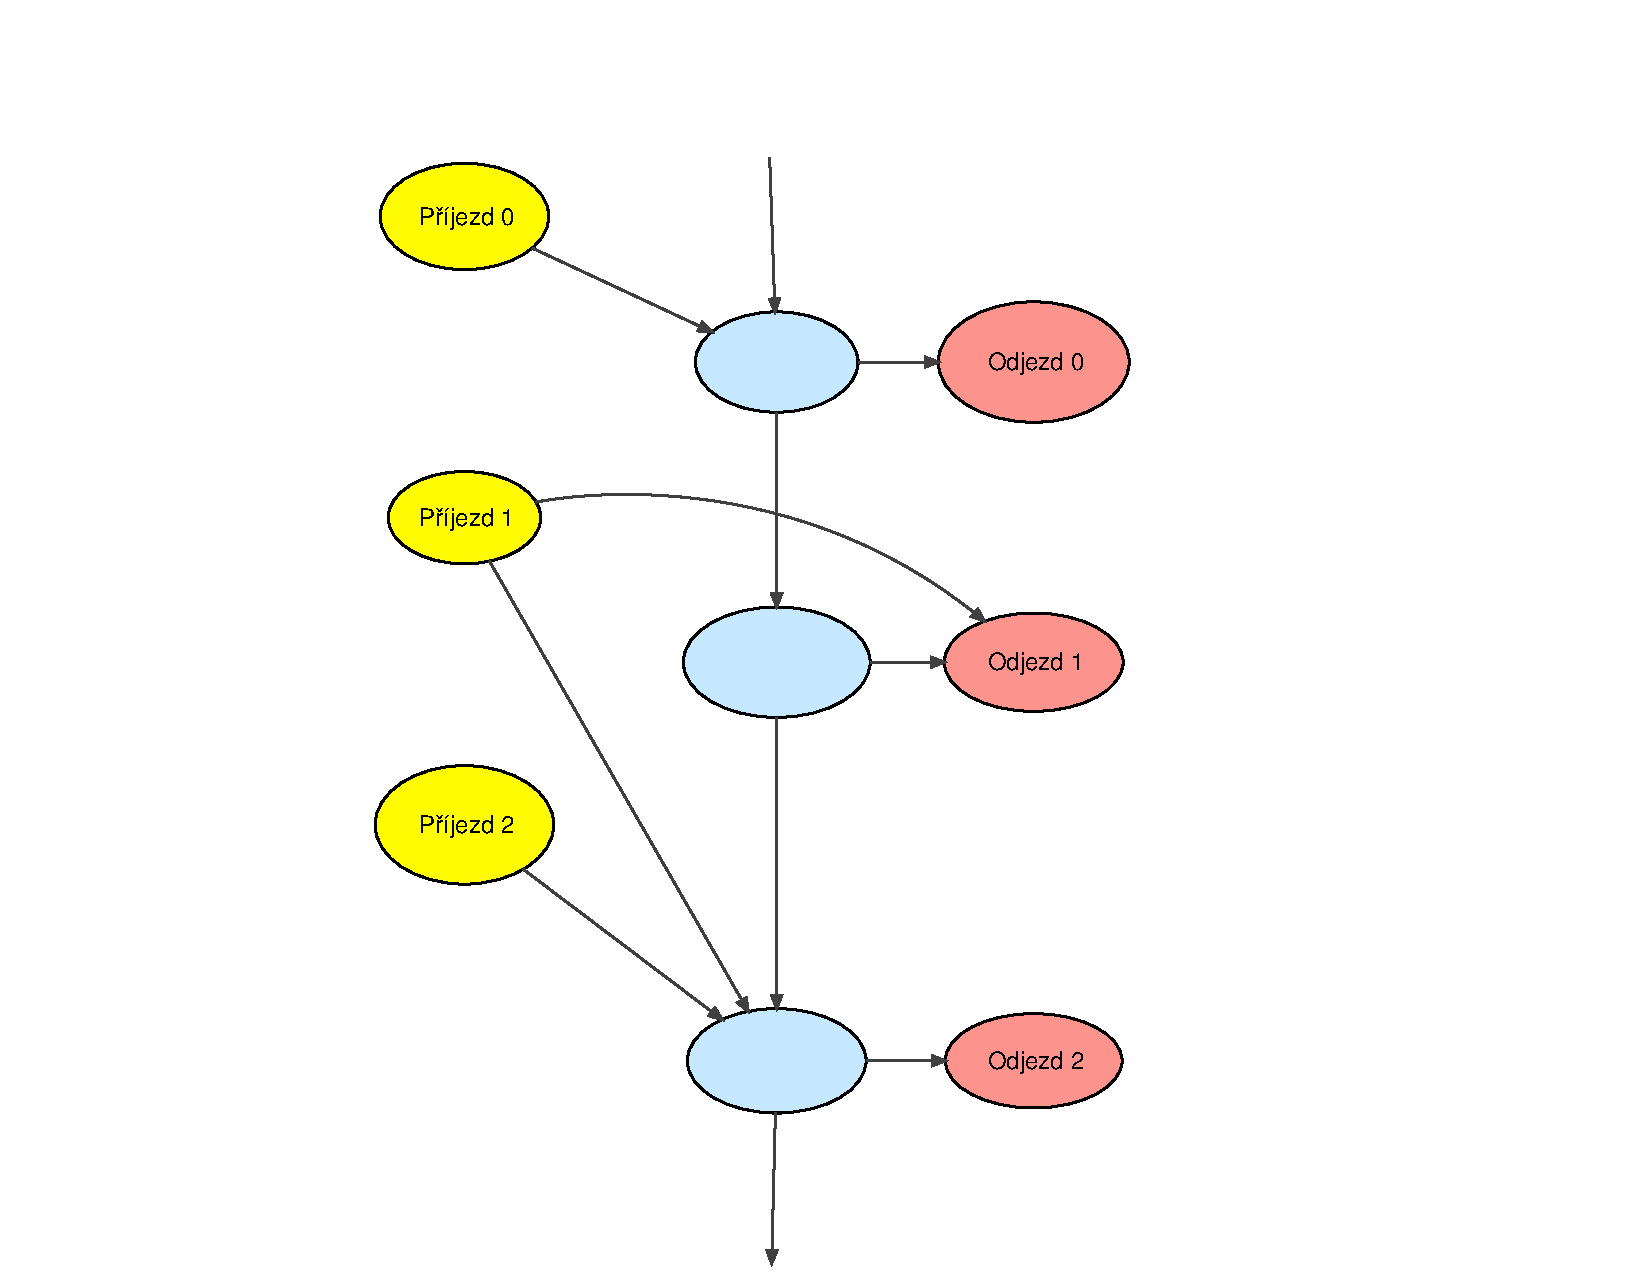
\includegraphics[width=\textwidth]{../img/time-expanded.pdf}
  \caption{Příjezdové (žlutě), odjezdové (červeně) a zastávkové (modře) vrcholy.
  Všimněte si, že z příjezdu 1 lze stihnout odjezd 1, ale jen proto, že jsou
  blízko sebe, obecný spoj odjíždějící ze zastávky v čase odjezd 1 bychom
  nestihli.}
  \label{fig:time-expanded}
\end{figure}

\section{Time-dependent modely}
Time-dependent modely\cite{time-dependent} se snaží odstranit problém
s~velikostí grafu hromadné dopravy. Místo toho, abychom měli pro každý spoj
zvláštní hranu, sdružíme spoje do linek, kde všechny spoje jedné linky mají
stejnou posloupnost zastávek. Vrcholy tentokrát budou jen jeden pro každou
zastávku. Hrany mezi zastávkami budou jedna pro každou linku, která danou
dvojici zastávek spojuje. V~takovémto grafu již nemůžeme vyhledávat pomocí
běžného průchodu grafem, potřebujeme mít upravenou funkci, která vyhledá
v~jednotlivých časech odjezdu pro každou linku nejbližší od okamžiku příjezdu do
zastávky. Tento přístup nevytváří grafy s~velkým počtem vrcholů a hran, navíc je
tato reprezentace snáze připojitelná do vyhledávacího grafu pro obyčejnou cestní
síť.

Existuje také varianta, která má jeden staniční vrchol a
pro každou linku projíždějící danou stanicí linkový vrchol. Tyto vrcholy jsou
pak propojeny přestupovými hranami a umožňují realističtější modelování
rozsáhlejších stanic a přestupů v~rámci nich. Ani tento model však nevyužívá
všech vlastností spojů MHD, jako je například to, že spoj má danou trasu a že
když na něj někde nastoupíme, tak snadno můžeme do dalšího vyhledávání přidat všechny
průjezdní stanice.  

\section{Contraction hierarchy}
Contraction hierarchy\cite{CH} je způsob předzpracování dat tak, aby následné
vyhledávání nemuselo procházet celý graf. U~cestní sítě tomu odpovídá obvyklý
postup při cestování -- nejprve cestujeme po místních silnicích, abychom se
dostali na silnice první třídy a dálnice, po těch pak dojedeme blízko cíle, kde
opět přecházíme na místní silnice, abychom dosáhli cíle. U~cestní sítě se
příprava dat provádí obdobně -- jsou nalezeny významné body, přes které
přecházíme na silnice vyšších tříd a cesty na dlouhé vzdálenosti jsou pak
rozděleny na hledání cesty do významných bodů a hledání cesty mezi nimi. Tato
hierarchie může mít i několik stupňů a cesty mezi významnými body jsou často
předpočítány.

Obdobně se dá vytvořit podobná hierarchie i u~hledání spojení MHD, kdy si
udržuji zkratky mezi uzlovými zastávkami a nemusíme pak prohledávat jednotlivé
mezilehlé zastávky, kde stejně nemůžeme na nic přestoupit. Problém této
reprezentace pro nás je s~přidáváním pěších tras, protože je potřeba mít všechny dopředu
spočítané. Předvýpočet je stejně tak problematický i u~cestní sítě, protože
předpokládá pevné nastavení cestovních rychlostí a preferencí cest, na základě
kterých jsou nalezeny uzlové body a vypočítány zkratky. Náš cíl je umožnit
uživateli tyto parametry si zvolit při hledání dle svých potřeb, proto pro nás
není tento model vhodný. 

\section{RAPTOR}
RAPTOR (Round-Based Public Transport Routing)\cite{RAPTOR} je oproti
time-dependent modelům založen na zcela odlišných myšlenkách a při svém běhu
nevyužívá algoritmy pro procházení grafu. RAPTOR se snaží využít co nejvíce vlastností,
kterými se odlišuje síť veřejné dopravy od obyčejné cestní sítě. Také umožňuje
snadno optimalizovat na počet přestupů.

Algoritmus pracuje po kolech. Každé kolo znamená nástup do dalšího dopravního
prostředku, celkově je tedy počet kol o~1 větší než maximální počet přestupů.
Algoritmus pracuje s~linkami. Každá linka má několik spojů, což jsou konkrétní
vozidla, která všechna projíždí stejnou posloupnost zastávek ve stejném směru. Každý spoj má
uloženy časy odjezdu z~jednotlivých zastávek, předpokládáme, že se dva spoje
jedné linky na trase nepředjíždí. Pro každou zastávku si pro každé kolo
pamatujeme, zda a kdy je dosažitelná pomocí kterého kola. Nedosažitelnost
zastávky reprezentujeme pomocí nastavení času příjezdu v~daném kole na $\infty$.

Na začátku jsou všechny zastávky ve všech kolech nedosažitelné. Nastavíme
výchozí zastávce čas dosažení v~prvním kole na zadaný čas odjezdu a spustíme
algoritmus. Ten postupně prochází linky po jejich zastávkách a pokud narazí na
dosažitelnou zastávku, tak najde nejbližší spoj linky, který z~dané zastávky
odjíždí po čase dosažitelnosti a tímto spojem se \uv{vydá} a průběžně upravuje
časy dosažitelnosti na dalších zastávkách. Pokud po cestě nalezne další
dosažitelnou zastávku, jako spoj z~této zastávky vybere z~původního spoje a
spoje navazujícího na původní čas dosažitelnosti ten, který odjíždí dříve. Takto
pokračuje až do konce linky. Po průchodu všech linek se všechny časy
dosažitelnosti zkopírují do dalšího kola a algoritmus se znovu spustí. Po
stanoveném počtu kol algoritmus skončí a u~jednotlivých zastávek je pro každé
kolo (odpovídající počtu přestupů $- 1$) uloženo, zda je s~daným počtem přestupů
dosažitelná a v~jakém čase. K~jednotlivým časům u~zastávek je vhodné si uložit
linku, která způsobila úpravu na daný čas, abychom byli schopni zrekonstruovat
spojení využité k~dosažení dané zastávky. 

Tento algoritmus je snadno implementovatelný a při vhodně zvolených datových
strukturách velmi rychlý a vhodně využívající keš. 

\subsection{Uložení dat}
\label{ch:reserse:raptor-data}
Pro rychlý výpočet a efektivní využití keše je potřeba mít vhodně uložená data.
Data stejného typu jsou vždy uložená v~poli za sebou. Pokud různé objekty mají
každý mít seznam stejného typu, jsou všechna data od všech objektů držena
v~jednom poli a každý objekt si drží počet svých prvků a odkaz na první z~nich.
Tímto má každý objekt vyhrazen svůj úsek a může s~ním efektivně pracovat. Tento
mechanismus nazveme \uv{polním mechanismem} a budeme na něj takto odkazovat ve
zbytku kapitoly.

Základem pro prohledávání je pole linek. Každá linka má odkaz na své zastávky a
na časy zastavení spojů v~zastávkách. Obojí je implementováno polním mechanismem
a rozdělení na zastávky a spoje zajišťuje snadnou možnost hledání spojů v~daný
čas. Časy zastavení spojů v~zastávkách jsou uspořádány v~poli za sebou podle
zastávek a pak podle času výjezdu spoje z~výchozí zastávky. Protože
předpokládáme, že se spoje nepředjíždí a všechny spoje jedné linky mají stejný
počet zastávek, na předchozí spoj snadno přejdeme skokem v~poli zastavení
o~počet zastávek linky vzad, následující spoj najdeme obdobným skokem vpřed. Také
je možné pro konkrétní zastávku a konkrétní čas použít jednoduše binární
vyhledávání pro nalezení nejbližšího spoje odjíždějícího po konkrétním čase. 

Pro vyhledávání z~konkrétní zastávky máme obdobně implementovány datové
struktury kolem zastávek. Zastávky jsou uloženy v~poli za sebou, každá si drží
seznam linek, které jí projíždějí, a seznam pěších přestupů z~dané zastávky. 
Obojí je reprezentováno polním mechanismem.   


\chapter{Zdrojová data}

Zdrojová data pro vyhledávač pochází ze dvou zdrojů. Prvním zdrojem jsou mapová
data, která obsahují silnice, cesty, budovy a další mapové prvky. Druhým zdrojem
jsou data o jízdních řádech, která obsahují linky, zastávky a spoje.

\section{Mapová data}
Mapová data jsou použita z projektu OpenStreetMap (OSM). Tato data neobsahují
informace o nadmořské výšce jednotlivých bodů, k doplnění nadmořské výšky jsou
použita data z projektu Shuttle Radar Topography Mission (SRTM), která jsou
lineárně interpolována pro získání nadmořských výšek jednotlivých bodů v mapě.
%TODO Kecy o OSM

\section{Jízdní řády}
Data o jízdních řádech jsou očekávána ve formátu General Transit Feed
Specification (GTFS), který je dobře specifikovaný a široce používaný ve světě.
Konkrétně pro testování byla použita data o pražské integrované dopravě od IPR
Praha\footnote{\url{http://opendata.iprpraha.cz/DPP/JR/jrdata.zip}}. Tato data
obsahují metro, tramvaje, autobusy a přívozy v Praze a okolí, bohužel neobsahují
integrované vlakové spoje.

GTFS je distribuováno jako archiv ZIP obsahující jednotlivé tabulky ve formátu
CSV. Význam jednotlivých tabulek je následující:
\begin{itemize}
\item {\em agency.txt} obsahuje informace o dopravcích na jednotlivých linkách.
V našem vyhledávání není používán.
\item {\em stops.txt} obsahuje informace o zastávkách. Zastávky jsou dvou typů.
Prvním typem je zastávkový stojan, který reprezentuje fyzické místo, kde
zastavuje nějaký spoj některé linky. Druhým typem je \uv{stanice}, která udává
oblast několika stojanů, obvykle stejného jména. Nemusí mít fyzickou
reprezentaci a slouží pro zobrazování v mapě a svázání logicky blízkých stojanů.
Protože stanice pro náš vyhledávač nenese důležitou informaci, využíváme pouze
zastávkové stojany (\TODO implementovat). Pro vyhledávání spojení využíváme
následující položky:
\begin{itemize}
	\item {\tt stop\_id} -- jednoznačný identifikátor zastávky
	\item {\tt stop\_name} -- název zastávky
	\item {\tt stop\_lat, stop\_lon} -- poloha zastávky
	\item {\tt location\_type} -- informace, zda jde o stojan, nebo stanici
\end{itemize}
\item {\em routes.txt} obsahuje informace o linkovém vedení. Pro vyhledávání
spojení využíváme následující položky:
\begin{itemize}
	\item {\tt route\_id} --
	\item {\tt route\_short\_name} -- 
	\item {\tt route\_type} -- 
\end{itemize}
\item {\em trips.txt} obsahuje informace o spojích. Tato tabulka slouží ke
svázání spoje (cesty konkrétního dopravního prostředku po posloupnosti zastávek
v daný čas), linky a množiny dní, kdy daný spoj jezdí. Pro vyhledávání využíváme
následující položky:
\begin{itemize}
	\item {\tt route\_id} -- 
	\item {\tt service\_id} -- 
	\item {\tt trip\_id} -- 
	\item {\tt } -- 
\end{itemize}
\item časy zastavení
\item kalendář
\end{itemize}


\chapter{Předzpracování dat}


\section{Příprava mapových dat}
Nejprve jsou stažena aktuální data pro Českou republiku, která jsou k~dispozici
s~denními aktualizacemi.\footnote{\url{osm.kyblsoft.cz/archiv/}} Z~těchto dat je
na základě nastavení vyříznut obdélník, který pokrývá zpracovávanou oblast. Poté
začneme data zpracovávat.

Nejprve jsou klasifikovány jednotlivé objekty. Klasifikují se uzly, hrany a
multipolygony, jiné typy relací nejsou v~současné době používány. Každý objekt
je klasifikován nějakým typem podle toho, jaké má tagy. V~rámci konfigurace lze
přidělit nějakému tagu (buď samotnému klíči, nebo dvojici klíč-hodnota) určený
typ s~danou prioritou. Objekt bude mít typ daný pravidlem s~nejvyšší prioritou,
které jeho tagy splňují. Pokud objekt nesplňuje žádné pravidlo, získá speciální
typ označující neklasifikovaný objekt.V dalším zpracování se již nehledí na
původní tagy ale jen na typ, který daný objekt má.

Současně s~klasifikací typu objektu se stejným způsobem určují hrany, které se
nachází na mostech a uzly, které jsou v~podzemí. Klasifikovaná data nahrajeme do
databáze a další kroky provádíme jako databázové operace. 

\subsection{Dělení dlouhých linií}
Protože chceme hledat co nejblíže od výchozího zadaného bodu, v~případě dlouhých
rovných ulic, které jsou reprezentovány pomocí lomených linií s~dlouhými úseky
by se nám mohlo stát, že by nejbližší bod od hledaného místa neležel na ulici,
kde jsme, ale na nějaké sousední, od které nás dělí pás budov. Proto dlouhé
úseky cest rozdělíme na menší podúseky (viz obr. \ref{fig:deleni}, čímž tento problém eliminujeme.
Rozdělení se nám také bude hodit pro vytváření zkratek, o~kterých pojednáváme
níže.

\begin{figure}
  \centering
    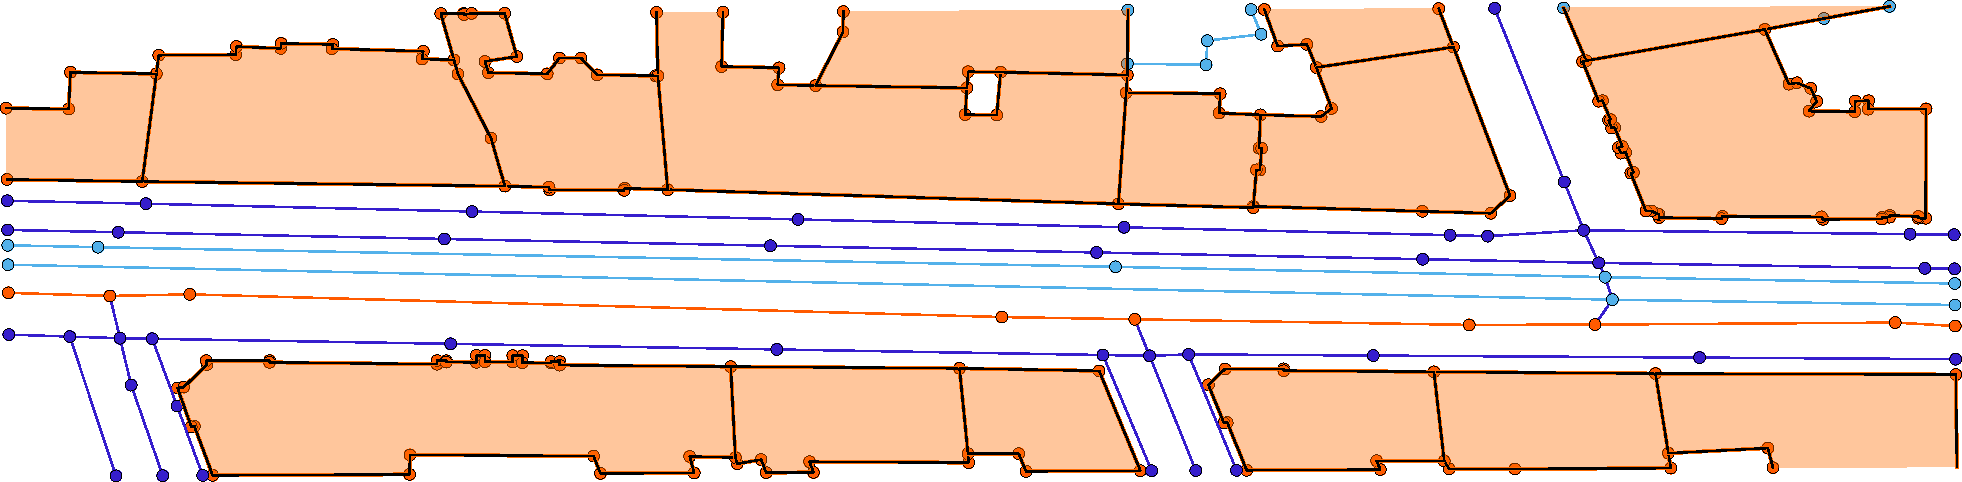
\includegraphics[width=0.75\textwidth]{../img/deleni.pdf}
  \caption{Rozdělení dlouhých linií (všimněte si, že jsou děleny jen pochozí
  linie)}
  \label{fig:deleni}
\end{figure}

\subsection{Překážky}
Pro další zpracování potřebujeme znát nejen cestní síť, ale i překážky, přes
které se nedá projít, jako jsou například domy, ploty a dálnice. V~tomto místě
se musíme vypořádat s~multipolygony. Protože multipolygony, které klasifikujeme
jako bariéry, jsou většinou budovy, které mají více částí nebo mají nádvoří,
nebo jiné překážky, uvnitř kterých neočekáváme velkou plochu, bereme
jako překážku jejich vnější obrys, případně obrysy. To nám sice způsobí, že
nebudeme moci vytvářet na vnitřních prostranstvích zkratky, ale to nám nevadí,
protože jednak mají vnitřní prostranství obvykle velmi malou plochu a nevede do
nich mnoho pěších cest, jednak vnitřní prostranství jsou buď zmapována
kompletně, nebo nedostatečně, tudíž by případné vytváření zkratek ve vnitřním
prostranství vedlo k~cestám, které by ve skutečnosti nebyly možné.

Výsledná množina překážek bude obsahovat vnější obrysy multipolygonů, další
polygonové objekty a liniové objekty.

\subsection{Body uvnitř objektů a body pod zemí}
Abychom mohli generovat zkratky, které budou průchozí i ve skutečnosti, je
potřeba určit, které body se nachází na volném prostranství na povrchu a které
se nacházejí pod zemí. Podzemní vrcholy jsme určili už v~rámci klasifikace.
Vrcholy uvnitř objektů jsme ztotožnili s~vrcholy, které se nachází uvnitř nějaké
překážky, protože překážky jsou pro nás takové objekty, přes které se nedá pěšky
projít napříč. Body, které se nacházejí na plášti překážky, jako vnitřní
neuvažujeme, protože se z~nich dá jít libovolným směrem, kde se nenachází
překážka.

\subsection{Zkratky}
Pro doplnění chybějících vazeb v~mapě používáme kromě cest v~mapových datech
již obsažených i automaticky generované zkratky. Zkratka spojuje dva pochozí
body na volném prostranství, které jsou nedaleko od sebe a úsečka mezi nimi,
reprezentující zkratku, neprotíná žádnou překážku. Dvojic bodů, které splňují
zadané podmínky, je ale velké množství a přidání všech zkratek by neúměrně
zvyšovalo velikost výsledných dat. Od počtu zkratek z~daného vrcholu přidávání
dalších zkratek má jen malý vliv na délky hledaných cest, proto jsou ze všech
možných zkratek náhodně vybrány jen některé a to tak, aby z~každého vrcholu
vycházelo průměrně omezené množství zkratek. Takto zachováme pozitivní vliv
zkratek na hledané cesty, ale zbytečně nezvětšujeme vyhledávací graf.
\begin{figure}
  \centering
    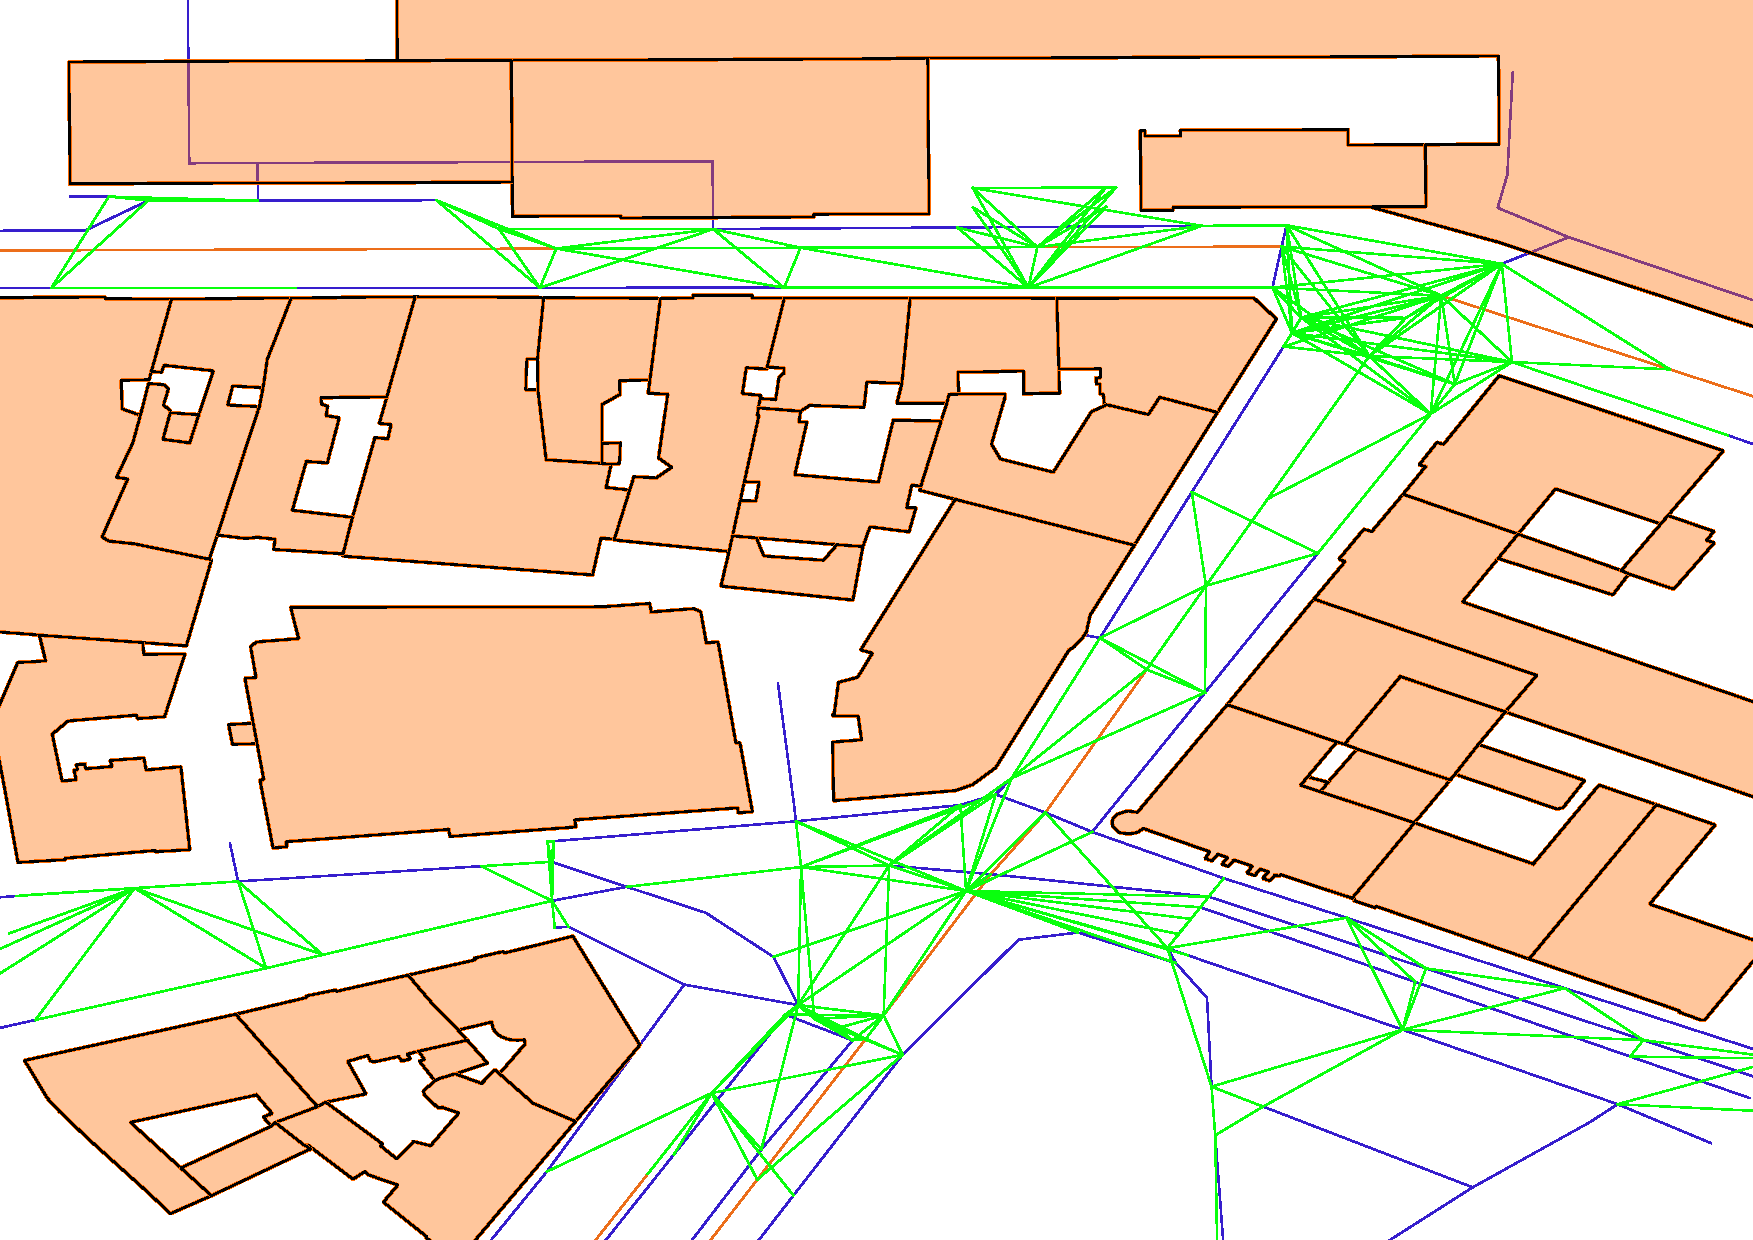
\includegraphics[width=0.5\textwidth]{../img/zkratky.pdf}
  \caption{Vygenerované zkratky mezi cestami (zeleně)}
  \label{fig:zkratky}
\end{figure}

\section{Příprava jízdních řádů}
Data z~jízdních řádů dostáváme ve formátu GTFS \cite{GTFS} a musíme je
upravit do formátu vhodného pro algoritmus RAPTOR \cite{RAPTOR}. V~rámci převodu
mezi formáty je potřeba respektovat specifické požadavky algoritmu RAPTOR a také
je potřeba připravit si informace potřebné pro propojení mezi zastávkami
v~jízdním řádu a zastávkami na mapě.

\subsection{Rozdělení linek}
Formát GTFS rozlišuje linky a spoje. Linka obsahuje všechny společné údaje a
jednotlivé spoje pak reprezentují jízdu vozidla dané linky mezi konkrétními
stanicemi, různé spoje jedné linky mohou projíždět různé posloupnosti stanic
(například spoje zatahující do vozovny, zkrácené vložené spoje, \dots).
Algoritmus RAPTOR ale vyžaduje, aby spoje konkrétní linky projížděly vždy
stejnou posloupnost zastávek. Abychom toho dosáhli, v~rámci předzpracování
najdeme všechny různé posloupnosti zastávek projížděné jednou linkou a vytvoříme
sublinky pro každou takovou posloupnost. Tyto sublinky zdědí společné údaje
z~původní linky a již splňují požadavky kladené algoritmem RAPTOR. 

\subsection{ID zastávek}
Zastávky mají dle specifikace GTFS jako ID použit obecný string. Data pro
pražskou MHD mají toto ID rozdělené na na část reprezentující zastávku a část
reprezentující konkrétní zastávkové stojany. Pro další zpracování je vhodné
zvolit číselný identifikátor, jednotlivé zastávky jsou očíslovány čísly od 0 do
počet zastávek $- 1$ a veškeré odkazy na konkrétní zastávky ve zpracovaných datech
používají právě tato čísla. Původní identifikátor je u~zastávky stále uložen
kvůli následnému párování (viz níže), ale již se pro vazbu mezi daty nepoužívá.

\subsection{Platnost jízdního řádu}
Ve formátu GTFS jsou linky, spoje a dny, ve kterých daný spoj jede, provázány
pomocí tabulky trips. V~předchozím odstavci jsme popsali rozdělení linek podle
toho, kudy spoje jedou, nyní využijeme, že každý spoj v~GTFS má právě jednu
množinu dní, kdy jede a tuto informaci si uložíme i u~jednotlivých spojů v~nově
vytvářeném formátu.

Místo dvojího způsobu záznamu, kdy daný spoj jede -- pomocí výčtu dnů v~týdnu a
seznamu výjimek -- si pro každou možnost, jak může nějaký spoj jet, uložíme
bitmapu platnosti a datum začátku a konce platnosti současného jízdního řádu. 
Bitmapa začíná první den platnosti a $i$-tý bit udává, zda i-tý den od začátku
platnosti daný spoj jede.  

\subsection{Podzemní stanice}
Při párování zastávek a pozic na mapě budeme potřebovat zvlášť ošetřovat
podzemní stanice, ze kterých se nelze vydat libovolným směrem, ale jen
eskalátorovým tunelem. V~rámci předzpracování označíme jako podzemní takové
zastávky, ve kterých jezdí metro. V~Praze takovýto předpoklad funguje správně,
protože všechny nadzemní stanice metra jsou zmapovány detailním způsobem, kdy
zpracování dat funguje korektně, pro jiná města s~jinou kvalitou zmapování by
bylo potřeba stanovit odlišná kritéria.


\section{Párování zdrojových dat}
Abychom moli plánovat spojení využívající jak pěší chůzi, tak jízdu MHD, je
potřeba data z~obou zdrojů vhodně provázat. Máme k~dispozici následující údaje:
\begin{enumerate}
\item OSM
\begin{itemize}
	\item jméno zastávky
	\item pozici zastávky
	\item ID zastávky (jen u~některých)
\end{itemize}
\item GTFS
\begin{itemize}
	\item jméno zastávky
	\item pozici zastávky
	\item ID zastávky
\end{itemize}
\end{enumerate} 
V~ideální připadě by bylo možné spárovat zastávky jednoduše dle ID, bohužel
v~OSM má ID jen několik zastávek, většinu zastávek je tedy potřeba spárovat jinak.
Nabízelo by se párování podle pozic a jmen zastávek, ale bohužel zastávky v~GTFS
jsou výrazně posunuté oproti OSM i skutečnosti, navíc ne všechny zastávkové
stojany jsou v~OSM vyznačeny, zvláště tam, kde je několik zastávkových stojanů
za sebou, například v~autobusových terminálech. Pokoušet se párovat zastávky
v~GTFS pouze na zastávky v~OSM by bylo velmi náročné s~nejistým výsledkem.
Využíváme proto toho, že v~OSM máme zmapované nejen zastávky, ale i cesty a
zastávkám v~GTFS vytváříme speciální vrcholy dle jejich zeměpisné pozice v~GTFS
a pomocí zkratek je spojujeme s~nejbližšími cestami (viz Obrázek
\ref{fig:zastavka}. Bod reprezentující zastávku pak v~mapových datech označíme
jako zastávku.

\begin{figure}
  \centering
    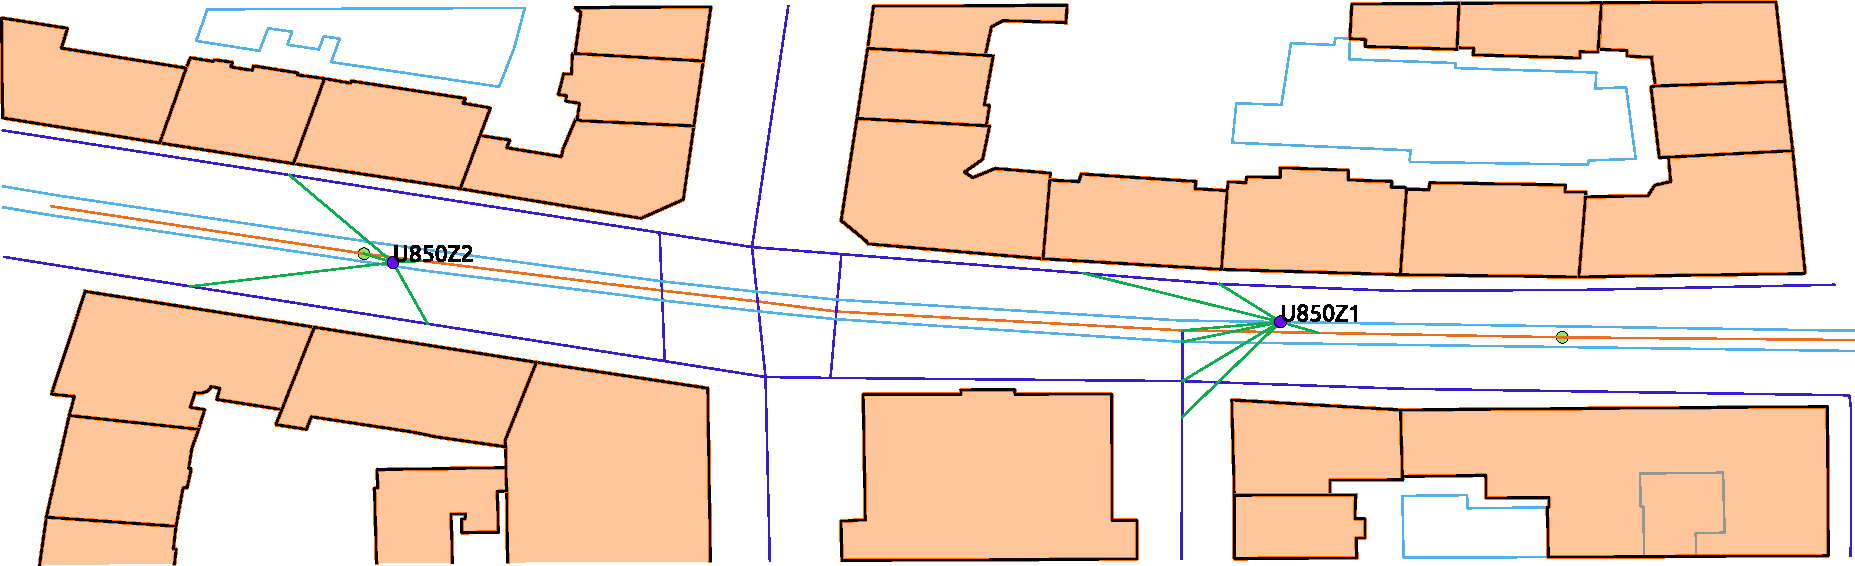
\includegraphics[width=\textwidth]{../img/tramvaj.pdf}
  \caption{Zkratky pro připojení tramvajové zastávky (zeleně)}
  \label{fig:zastavka}
\end{figure}

Pro zastávky z~GTFS, pro které máme v~OSM odpovídající ID, použijeme polohu
z~OSM a zkratky k~cestní síti hledáme z~této polohy. Zkratky jsou i zde potřeba,
protože dle pravidel OSM \cite{OSM} se zastávka umisťuje na místo, kde zastavuje
vozidlo, což například u~tramvají je bod na kolejích, které ale pro pěší
plánování nepoužíváme, tudíž je potřeba najít vhodný blízký bod v~cestní síti.

Zvláštní pozornost je potřeba věnovat u~párování zastávek metra. V~současné
chvíli je metro v~Praze zmapované dvěma způsoby. První způsob (viz obrázek 
\ref{fig:metro-detail}) je novější a
přesnější, jsou při něm zmapována nástupiště a eskalátorové tunely. Při tomto
podrobném mapování jsou také přidána ID stanic, tudíž je možné stanice jednoduše
spárovat a hledat cestu od hrany nástupiště. Častějším způsobem je ale starší
způsob (viz obrázek \ref{fig:metro-hrube}), kdy je stanice metra pouze bod, od
kterého vede eskalátorový tunel na
povrch. Tento eskalátorový tunel je pouze virtuální spojka, neodpovídá reálné
poloze podzemních tras. Takovéto stanice rovněž nemají přiřazená ID. U~těchto
stanic používáme polohu z~GTFS a zkratky spojující zastávku s~cestní sítí
hledáme do blízkých míst, která jsou v~podzemí, což vede k~poměrně dobré
aproximaci přístupu do metra. Jak bude postupovat mapování stanic metra, bude
tento typ stanic postupně eliminován a dojde ke zpřesnění navigace při
přestupech.

\begin{figure}
  \centering
    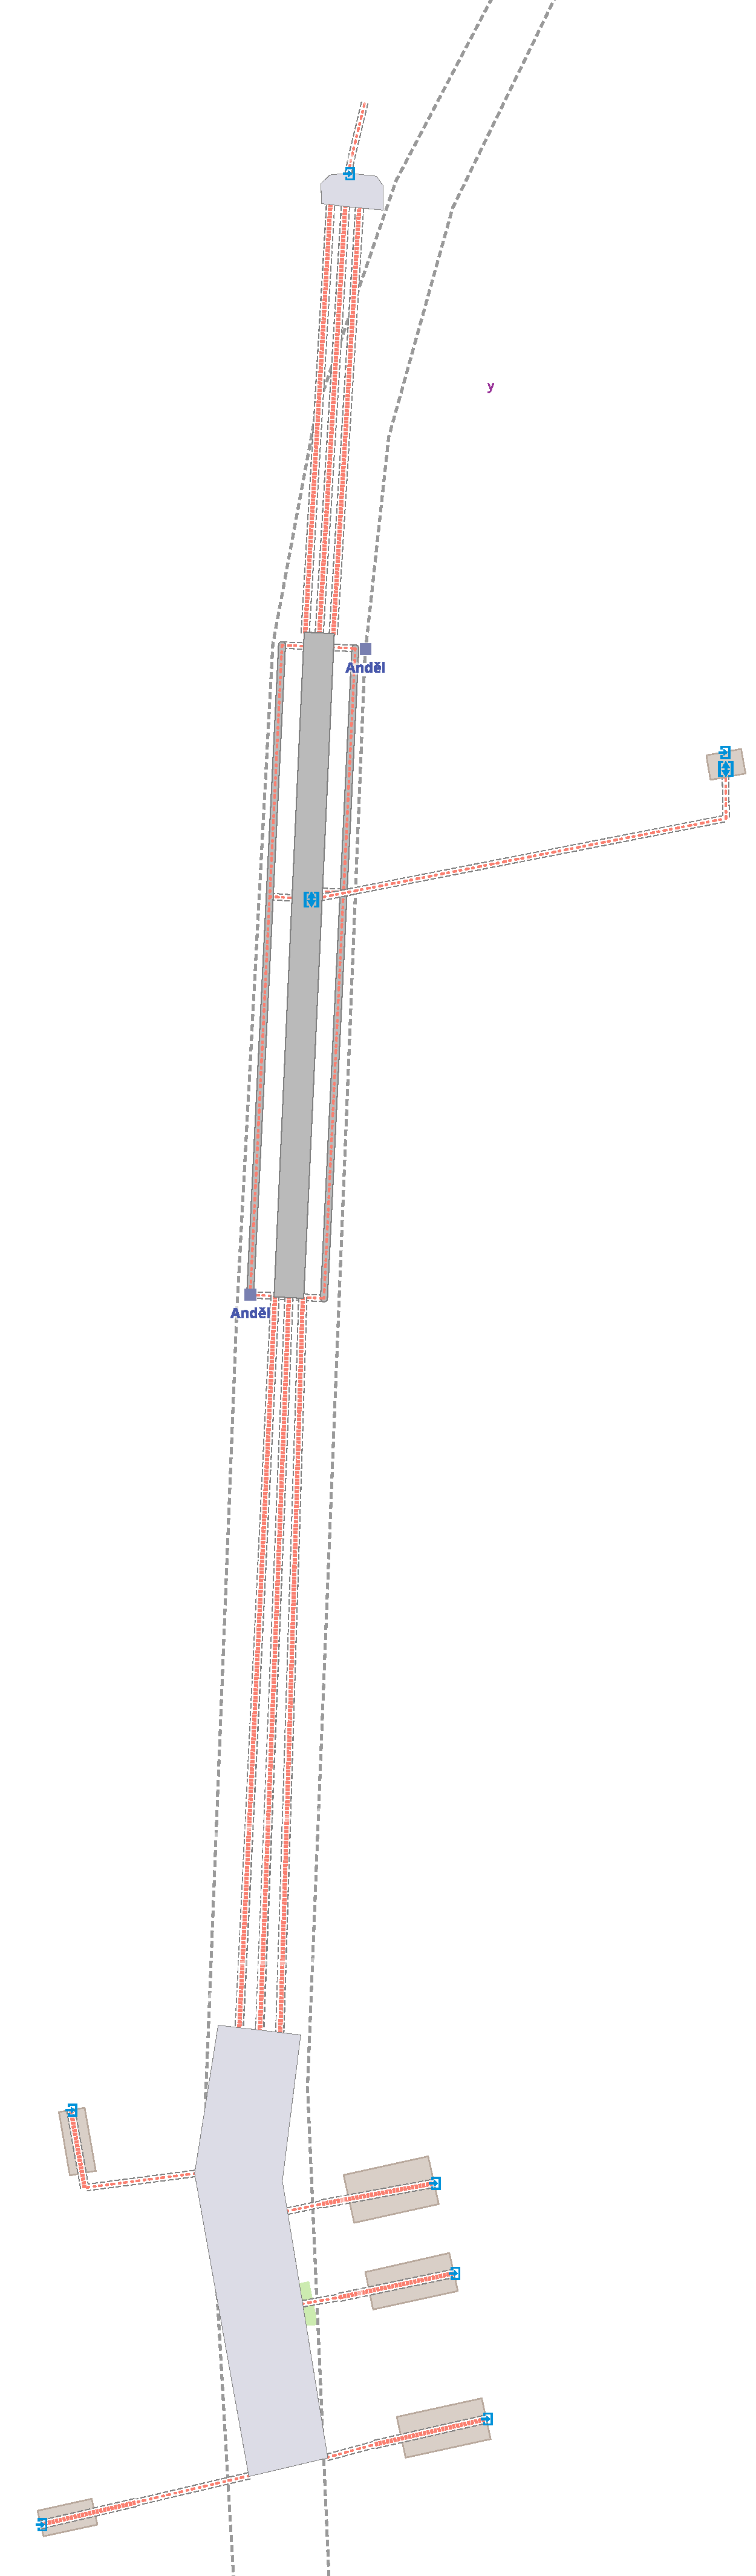
\includegraphics[height=0.99\textheight]{../img/andel.pdf}
  \caption{Detailně zmapovaná stanice metra Anděl}
  \label{fig:metro-detail}
\end{figure}

\begin{figure}
  \centering
    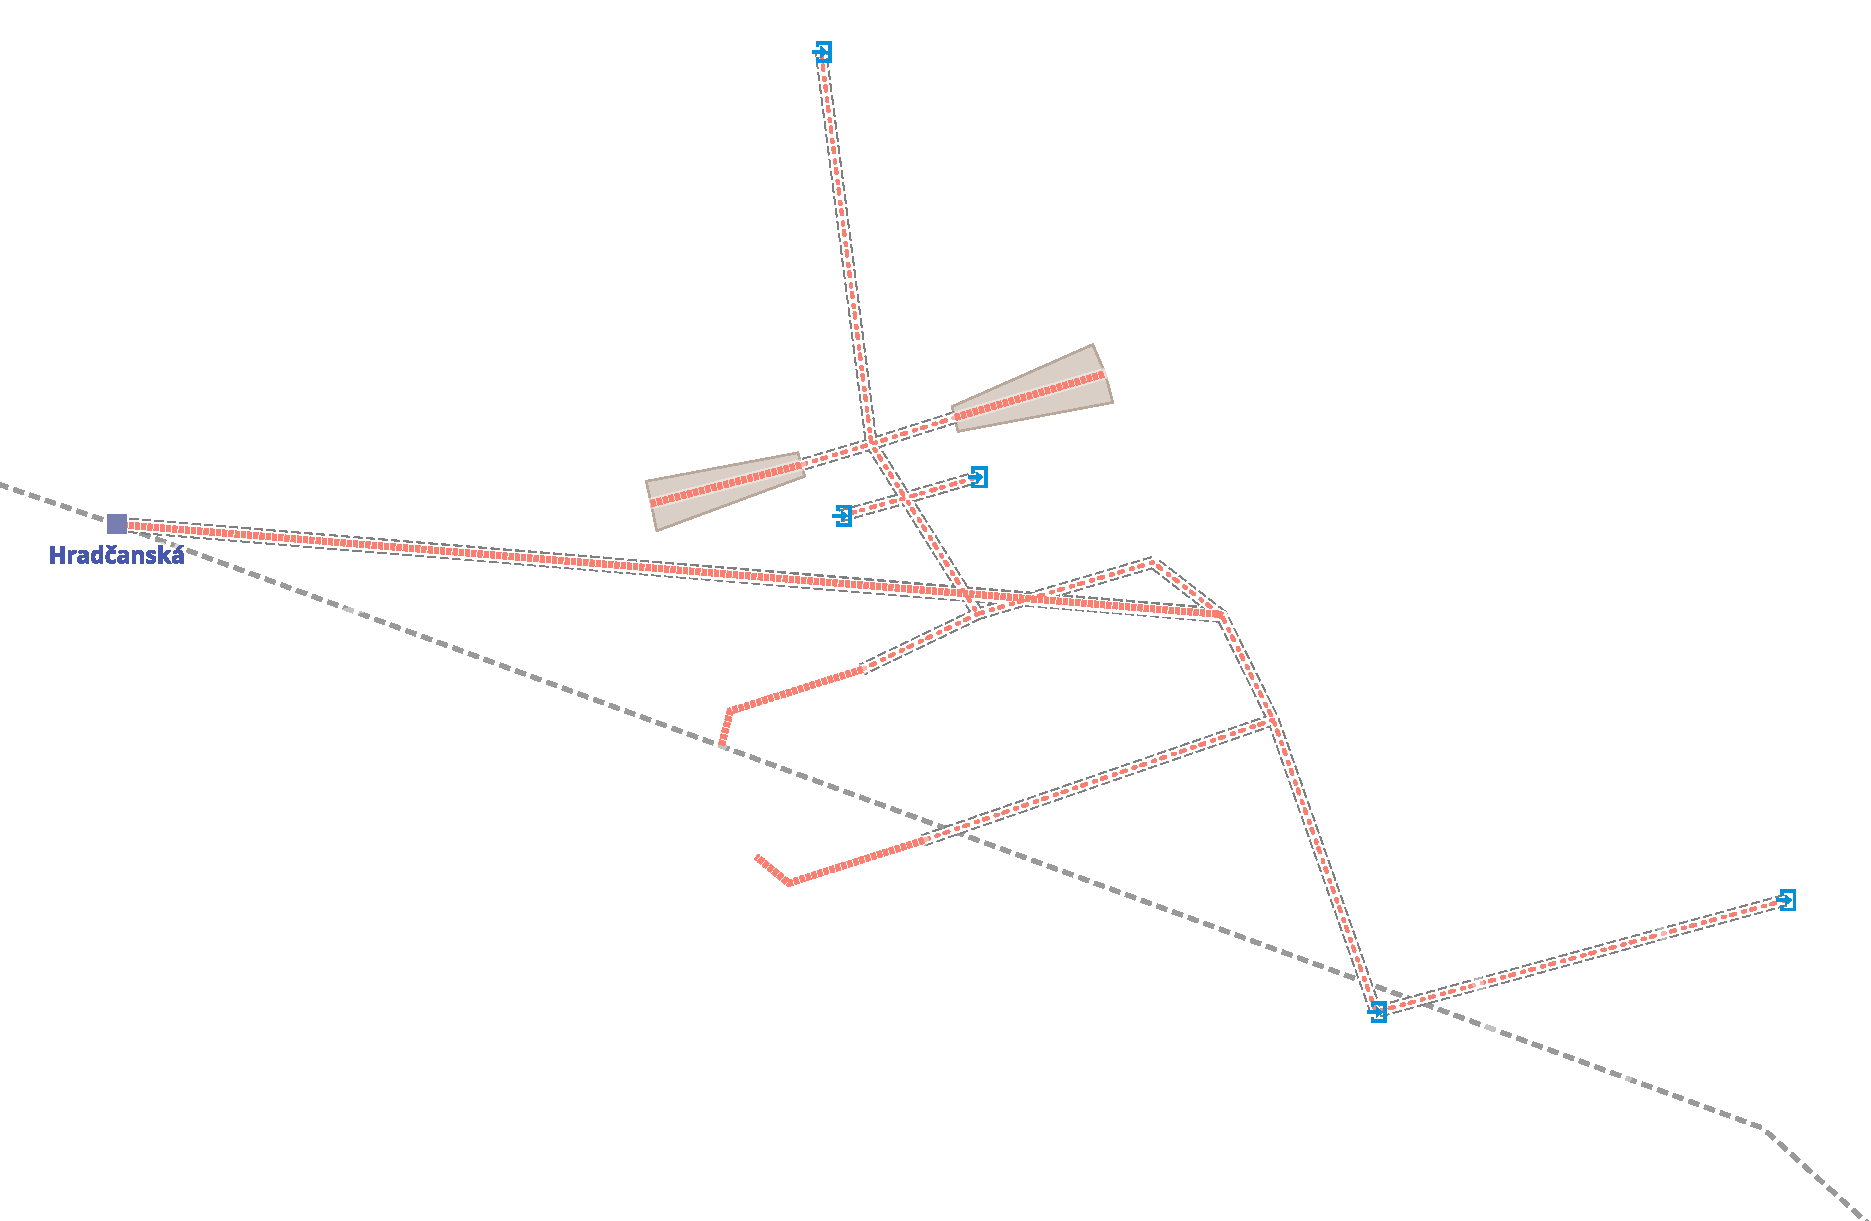
\includegraphics[width=\textwidth]{../img/hradcanska.pdf}
  \caption{Stanice metra Hradčanská zmapovaná starším způsobem}
  \label{fig:metro-hrube}
\end{figure}

Vždy jsou preferovány zastávky a stanice zmapované přesněji, které mají ID,
stačí tedy vylepšovat mapu a při dalším předzpracování dat se nově zmapované
zastávky dostanou i do vyhledávače.


\chapter{Vyhledávání trasy}
V~připravených datech je možné opakovaně vyhledávat spojení. Ke hledání spojení
se využívá Dijkstrův algoritmus a RAPTOR. Nejprve se naleznou nejbližší vrcholy
grafu k~zadaným výchozím a cílovým souřadnicím. Poté se začne Dijkstrovým
algoritmem prohledávat graf pěších cest. Pokud při prohledávání narazíme na
zastávku MHD, provedeme z~této zastávky jedno kolo algoritmu RAPTOR, najdeme
tedy všechny zastávky, kam se umíme bez přestupu dostat z~dané zastávky. Všechny
tyto zastávky přidáme do fronty Dijkstrova algoritmu s~časem dosažení rovným
času příjezdu do dané stanice. 

Při běhu algoritmu počítáme pro každou cestu její penaltu -- čím větší má
cesta penaltu, tím horší pro nás je. Samotný Dijkstrův algoritmus bere vrcholy
podle času dosažení. Po nalezení nejrychlejší cesty se nezastaví, ale počítá
dokud nezpracovává vrchol o~nějaký koeficient horší, než je nejkratší cesta. 
Tento postup byl zvolen, protože při hledání cesty se chce uživatel dostat z~výchozího
do cílového bodu co nejrychleji, ale má nějaké preference na to, jak by měla
cesta vypadat. Pokud vyhledáváme podle času, dostane uživatel jednak nejkratší
cestu, jednak alternativní cesty, které jsou sice o~něco delší, ale více splňují
představy uživatele o~optimální cestě.

Pokud bychom během vyhledávání udržovali všechny trojice (vrchol, čas příjezdu,
penalta), byl by procházený stavový prostor obrovský a vyhledávání by bylo velmi
náročné na paměť i čas. Pro redukci stavového prostoru uvažujeme uspořádání pro
každý vrchol, kde spojení $A$ je horší než spojení $B$, pokud $A$ má pozdější
čas dosažení vrcholu a vyšší penaltu než $B$. V~takovém případě spojení $A$ do
fronty otevřených vrcholů vůbec nepřidáváme, případně ho zahodíme, když na něj
ve frontě narazíme. Takovéto situaci říkáme, že spojení $B$ majorizuje spojení~$A$

\section{Redukce duplicitních tras}
I~přes uvažování pouze nemajorizovaných spojení získáme mnoho spojení, které se
liší jen drobnými změnami v~pěších částech trasy. Pro skutečnou cestu podle
nalezeného spojení nemají tyto drobné rozdíly význam, proto se snažíme takovéto
duplicity ignorovat. Základním předpokladem, který učiníme, budiž to, že pokud
se dvě spojení liší v~použitém spoji MHD, tak chceme obě zobrazit. Dále se tedy
zabýváme jen spojeními, které mají shodné části využívající MHD. Jako duplicitní
spojení bychom rádi označili taková spojení, která vedou celou cestu blízko
sebe.Takovéto pravidlo je ale časově náročné implementovat, proto místo něj použijeme
zjednodušenou variantu.

Vezmeme pouze pěší části spojení a porovnáváme vždy
odpovídající pěší části proti sobě. Procházíme hrany a hledáme, kde se liší.
Zapamatujeme si index první takovéto hrany. Pak projdeme úsek od konce a opět
hledáme první hranu, kde se liší. Tímto máme ohraničený úsek, kde se cesty liší.
Podíváme se u~obou cest na vrchol uprostřed tohoto úseku a pokud jsou tyto
vrcholy příliš blízko sebe, označíme úsek jako duplicitní. Pokud mají dvě
spojení všechny pěší úseky duplicitní, jedno ze spojení zahodíme. Idea je, že
pokud se dvě cesty liší v~nějakém úseku, tak uprostřed tohoto úseku budou od
sebe nejdál. Toto pravidlo sice může eliminovat i cesty, které jsou odlišné a
potkávají se zrovna uprostřed, ale to se nestává často a pravidlo lze
implementovat v~lineárním čase.

\chapter{Implementace}
Pro implementaci programu převádějícího OSM data do formátu vyhledávacího grafu
jsme zvolili v~první části Python, protože pro něj existuje široké množství
knihoven, které nám pomohly při řešení jednotlivých dílčích problémů. Při
vytváření spojek mezi cestami a jejich následné kontrole již ale nedostačoval,
proto jsme tuto a další části implementovali v~jazyce C. Mezi těmito částmi
předáváme data pomocí Protocol Bufferu v~souboru. Vyhledávání je také
implementováno v~jazyce C kvůli rychlosti a paměťové nenáročnosti.

\section{Použité knihovny a pomocné programy}
Během implementace programu pro přípravu dat jsme se snažili použít co nejvíce
již existujících knihoven a programů pro jednotlivé řešené problémy. Všechny
tyto knihovny a programy jsou nutné pro spuštění a používání našeho programu. 

\medskip
\noindent Používáme tyto pomocné programy, údaj v závorce udává licenci:
\begin{itemize}
	\item Výřez s~městem z~dat pro republiku vyrábíme pomocí {\tuc
	Osmconvert} (GNU AGPL).\\
	\url{http://wiki.openstreetmap.org/wiki/Osmconvert}
	\item Pro práci s~Protocol Buffery v~Pythonu využíváme třídy generované
	kompilátorem {\tuc protoc} (BSD New).\\
	\url{http://code.google.com/p/protobuf/}
	\item Pro práci s~Protocol Buffery v~C využíváme funkce a struktury
	generované kompilátorem {\tuc protobuf-c} (BSD 2-Clause).\\
	\url{https://github.com/protobuf-c/protobuf-c}
\end{itemize}

\noindent V~programech napsaných v~Pythonu využíváme následující knihovny:
\begin{itemize}
	\item Na parsování konfiguračních souborů používáme {\tuc PyYAML}
	(MIT).\\
	\url{http://pyyaml.org/wiki/PyYAML}
	\item Na parsování OSM XML používáme {\tuc imposm.parser} (Apache).\\
	\url{http://imposm.org/docs/imposm.parser/latest/}
	\item Souřadnice konvertujeme pomocí {\tuc pyproj} (MIT).\\
	\url{http://code.google.com/p/pyproj/}
	\item Pro hledání komponent grafu využíváme {\tuc networkx} (BSD).\\
	\url{http://networkx.github.io/}
\end{itemize}

\noindent V~programech napsaných v~C využíváme následující knihovny:
\begin{itemize}
	\item Datové struktury, dynamická pole a další funkce zajišťuje
	{\tuc LibUCW} (GNU LGPL).\\
	\url{http://www.ucw.cz/libucw/}
	\item Výpočty se zeměpisnými souřadnicemi provádí {\tuc PROJ.4} (MIT).\\
	\url{http://trac.osgeo.org/proj/}
\end{itemize}

Program osmconvert je již zahrnut ve zdrojovém kódu, ostatní knihovny je
potřeba nainstalovat zvlášť.

\section{Datové struktury}
V~průběhu celé přípravy vyhledávacích dat často využíváme několik struktur,
které nyní popíšeme. Datové struktury využívané jen v~konkrétních případech
popíšeme u~těchto případů.

Při přípravě dat používáme několik {\tuc hešovacích tabulek}. Často potřebujeme
získat uzel respektive cestu s~konkrétním identifikátorem, pro tento účel nám
slouží tabulky \verb|nodesIdx| respektive \verb|waysIdx|. V~Pythonu jsou
reprezentovány typem slovník, v~C využíváme součást knihovny LibUCW
\verb|hashtable|. V~obou případech je klíčem OSM identifikátor objektu a
hodnotou index do pole uzlů resp. cest, kde je daný objekt uložen.

U~každé cesty je v~datech uložen seznam uzlů, přes které prochází. Je ale vhodné
mít i pro každý uzel uložen seznam cest, na nichž leží. Pro tento účel
máme seznam \verb|nodeWays|. Je to seznam seznamů, kdy pod indexem $i$ je seznam
všech identifikátorů cest, které prochází uzlem na pozici $i$ v poli všech uzlů.
V~Pythonu jde o~seznam seznamů, v~C je to rostoucí pole rostoucích polí
z~LibUCW.

Během zpracování hledáme uzly blízké daným uzlům. Abychom pro každé takové
hledání nemuseli procházet všechny uzly, vytvoříme si na začátku {\tuc mřížku}.
Tato mřížka dělí plochu mapy na čtverce $20 \times 20$\,m a v~každém čtverci si
uložíme seznam identifikátorů vrcholů, které v~něm leží. Poté nám při hledání
sousedů bodu stačí zjistit, do kterého čtverce patří, a následně prohledat jen
několik okolních čtverců.

Mřížka je vhodnou strukturou pro rozdělení plochy, protože zástavba ve městě je
poměrně homogenní, tudíž zde nejsou příliš velké volné plochy, kde bychom
zbytečně plýtvali pamětí, ani místa, kde by počet bodů ve čtverci mřížky byl
obtížný na zpracování.

V~Pythonu se jedná o~třídu \verb|Raster|, která při vytvoření vyrobí mřížku
z~mapy. Mřížka je uložena v~atributu \verb|raster|, třída má metodu
\verb|getBox(x,y)|, která pro bod se souřadnicemi $(x,y)$ vrátí tuple se
souřadnicemi buňky, ve které se bod nachází. Mřížka \verb|raster| je seznam
seznamů seznamů.

V~C je mřížka reprezentována strukturou \verb|raster_t|. Samotná mřížka je prvek
\verb|raster| této struktury. V~souboru \verb|raster.h| jsou definovány funkce
pro práci s~mřížkou. Funkce \verb|makeRaster(map_t map)| vyrobí z~mapy mřížku a
vrátí ji. Funkce \verb|getRasterBox(raster_t raster, int64_t x, int64_t y)|
dostane jako paramter mřížku a souřadnice bodu a vrátí pole se dvěma prvky --
souřadnicemi buňky, kde se bod nachází. Mřížka \verb|raster| je reprezentována
polem polí rostoucích polí z~knihovny LibUCW.

\medskip


\section{Stažení dat OSM}
Abychom mohli připravovat data pro vyhledávání, musíme nejprve získat data OSM
pro dané město. O~tuto činnost se stará skript \verb|prepare.sh|, který stáhne
data pro celou Českou republiku a pomocí programu \verb|osmconvert| z~ní vyřízne
obdélník s~městem. Ten uloží jako \verb|praha.osm|\footnote{Program byl
připravován pro vyhledávání tras po Praze, proto soubory obvykle obsahují název
praha.} k~dalšímu zpracování.

\section{Příprava dat SRTM}
Kromě dat OSM potřebujeme i údaje o výškách z projektu SRTM. Protože tato data
se, narozdíl od dat OSM, nebudou aktualizovat, není pro jejich stažení skript,
ale je nutné do složky \verb|osm| nahrát soubory \verb|.hgt|, které pokrývají
obdélník s městem. Pomocí programu \verb|merge-srtm| se \verb|hgt| soubory spojí
do jedné velké tabulky, která je uložena jako \verb|heights.txt|. Její první
řádek obsahuje rozsah pokrývaný SRTM tabulkou a další řádky pak obsahují tabulku
výšek.

\section{Klasifikace dat}
Před dalším zpracováním potřebujeme data OSM převést do formátu pro přípravu dat (premap).
K~tomuto účelu slouží program \verb|parse.py|, který si načte konfigurační soubory
a podle nich rozdělí jednotlivé uzly a cesty do kategorií. Současně také přidá k
uzlům údaje o nadmořské výšce a jejich souřadnice převede do UTM. Následně smaže 
všechny uzly, které neleží na žádné cestě, a uloží data do souboru ve formátu 
formátu premap.

Konfigurační soubory jsou soubory ve formátu YAML \cite{yamlspec}. Používají se následující
konfigurační soubory:
\begin{itemize}
	\item \verb|types.yaml| pro rozdělení cest a multipolygonů do
kategorií 
	\item \verb|area.yaml| pro určení, zda je daný objekt plochou
	\item \verb|tunnel.yaml| pro určení, zda je daný objekt tunelem,
	průchodem či jinou podobnou stavbou
	\item \verb|bridge.yaml| pro určení, zda je daný objekt mostem nebo na
	nějakém mostě leží
\end{itemize}

Konfigurační soubory mají následující formát:
\begin{verbatim}
BARRIER: 
    barrier : "*"
    waterway:
        - river
        - canal
WATER:
    waterway:
        - riverbank
        - stream
\end{verbatim}
Konfigurační soubor se skládá z~několika mapování, u~každého klíč určuje, jaká
kategorie resp. hodnota se přiřadí, hodnotou mapování první úrovně jsou mapování
druhé úrovně, které určují, za jakých podmínek se hodnota přiřadí. Přiřazuje se
vždy, když je splněna alespoň jedna podmínka. 

V~mapování druhé úrovně je klíčem vždy klíč vlastnosti objektu OSM. Hodnota může
být dvou druhů. Buď je to \verb|"*"|, pak stačí, že se shoduje klíč vlastnosti
OSM a na hodnoty se nehledí, nebo je hodnota mapování seznam hodnot objektu OSM.
Pokud má objekt OSM pro daný klíč jednu z~těchto hodnot, je  podmínka splněna. 

V~příkladu rozdělujeme do kategorií \verb|BARRIER| a \verb|WATER|. Pokud má
objekt OSM nějaký atribut s~klíčem \verb|barrier|, je tomuto objektu přiřazena
kategorie \verb|BARRIER| nezávisle na hodnotě tohoto klíče. Obdobně je jako
\verb|BARRIER| označen objekt OSM, který má atribut s~klíčem \verb|waterway| a
hodnotou \verb|river|. Pokud má ale objekt atribut s~klíčem \verb|waterway| a
hodnotou \verb|stream|, je klasifikován jako \verb|WATER|.

Při procházení uzlů jim přiřazujeme ze SRTM výšku a převádíme jejich souřadnice
do UTM. Pomocí metody \verb|calcHeight| spočítáme nadmořskou výšku daného uzlu a
následně jeho souřadnice převedeme do UTM. Navíc {\tuc vynásobíme souřadnice UTM
desíti}, čímž bude jednotkou 10\,cm. Taková přesnost nám stačí a můžeme všechny
výpočty provádět v~celých číslech.

Následně vytvoříme hešovací tabulku \verb|nodeWays| a jejím průchodem zjistíme, které
uzly neleží na žádných cestáchi, a tyto uzly smažeme. Nakonec převedeme data do
formátu premap a uložíme jako soubor \verb|praha-pre.pbf| do složky \verb|data|.

\section{Převod multipolygonů na cesty}
S~multipolygony se v~původní formě pracuje obtížně, protože se jejich obvod
skládá z~neseřazených cest. Pro naše účely se hodí vytvořit cesty reprezentující
obvod multipolygonu. Těchto cest může být více, protože multipolygon se může
skládat z~více komponent. 

Pro každý multipolygon si vytvoříme seznam všech vnějších cest. Pak vytvoříme
seznam sousedů \verb|neighs|, který pro každý uzel na některé z~vnějších cest
obsahuje jeho sousedy na těchto cestách. Ve správném případě by takto měl každý
uzel mít dva sousedy. Pokud tomu tak není, skončíme s~chybou. Poté vybereme
jeden uzel na obvodu a postupujeme po jeho sousedech, dokud se do něj opět
nevrátíme. Použité cesty smažeme ze seznamu všech cest a opakujeme, dokud nějaké
cesty zbývají. Pokud se vrátíme na vytvářenou cestu mimo první vrchol, skončíme
s~chybou.

\section{Spojení budov}
Při spojování bloků budov do jejich obrysu nejprve vytvoříme graf sousednosti
budov. Pro jeho reprezentaci použijeme knihovnu \verb|networkx|. Jednotlivé
budovy budou vrcholy v~grafu, pokud budovy sousední, bude mezi jejich vrcholy
hrana. Graf sousednosti vytváříme funkcí \verb|makeNeighGraph|.

Do grafu nejprve přidáme všechny budovy jako vrcholy. Následně procházíme
všechny uzly a u~každého zkoumáme cesty, které jím prochází. Pokud jde jen
o~budovy, pak mezi první budovou a všemi ostatními vytvoříme v~grafu hrany. Pokud
mezi cestami je i nějaká, která není budovou, pak jsou všechny sousední budovy
označeny za vadné a hrany nepřidáváme.

Když máme graf vytvořen, procházíme ve funkci \verb|mergeComponents| jednotlivé
jeho komponenty a ze všech cest v~komponentě, které nejsou vadné, se pokoušíme
vytvořit cestu. Pokud se to povede, přidáme ji mezi cesty a původní cesty
jednotlivých budov vložíme do seznamu ke smazání. Nakonec funkcí
\verb|removeMerged| smažeme všechny budovy, které jsme nahradili jejich obvodem.

Když vytváříme cestu z~obvodu bloku budov pomocí funkce \verb|mergeWays|,
postupujeme obdobně jako při převodu multipolygonů na cesty. Vytvoříme si seznam
\verb|neighs|, který obsahuje pro každý bod na některé ze spojovaných cest
všechny jeho sousedy. Tentokrát ale může být sousedů více a je potřeba vybrat
toho správného. Setřídíme si tedy uzly podle souřadnic lexikograficky a
nejjižnější z nejzápadnějších vezmeme jako první uzel obvodu.  Protože žádný
západnější ani jižnější bod neexistuje, bude tento uzel zcela jistě na obvodu.
Nyní najdeme druhý uzel na obvodu. Vybereme mezi sousedy prvního uzlu ten, který
svírá s~úsečkou vedoucí z~prvního uzlu na jih nejmenší úhel. Žádný uzel přímo na
jih od prvního není, proto všechny úhly budou nenulové. Uzel pod nejmenším úhlem
bude druhým na obvodu.

Pokud máme první dva body na obvodu, stačí nám již jen ze sousedů aktuálně
zpracovávaného uzlu vybrat ten uzel, který svírá s~předchozím a aktuálním uzlem
nejmenší vnější úhel a takto pokračovat, dokud se nevrátíme do prvního uzlu.

Jestliže počet uzlů je menší než tři, nejde o~korektní plochu a je vrácena chyba.
Rovněž pokud během průchodu po obvodu dojdeme podruhé do jiného než prvního bodu
na obvodu, například pokud se dvě cesty dotýkají rohem, vrátíme chybu.
% TODO: Obrázky

\section{Rozdělení dlouhých úseků}
Dlouhé přímé cesty mívají i úseky mezi uzly dlouhé. V~případě, že například
v~polovině tohoto úseku silnice končí souběžný chodník, chceme navázat cestu
z~chodníku na silnici spojkou. Protože spojky chceme mít krátké, hodí se nám mít i
krátké úseky mezi uzly a tím mít možnost kdekoli podél cesty na ni udělat
spojku. Projdeme tedy všechny cesty a na každé kontrolujeme délky úseků. Pokud
najdeme úsek delší než 30 metrů, rozdělíme ho po 20 metrech vytvořením nových
uzlů vložených mezi stávající.

\section{Výpočet průsečíku úseček}
V následujících částech budeme často počítat průsečík úseček. Nyní odvodíme
vzorec pro výpočet průsečíku přímek, pro úsečky stačí jen navíc kontrolovat,
jestli nalezený průsečík leží na obou úsečkách.


Mějme dvě přímky $p,q$ a body $A,B,C,D$ takové, že $A,B \in p$ a $C,D \in q$.
Nechť body mají následující souřadnice: $A=[x_1,y_1], B=[x_2,y_2], C=[x_3,y_3]$
a $D=[x_4,y_4]$. Hledáme průsečík $P = [x,y]$ přímek $p$ a $q$.

\begin{figure}[h]
	\centering
	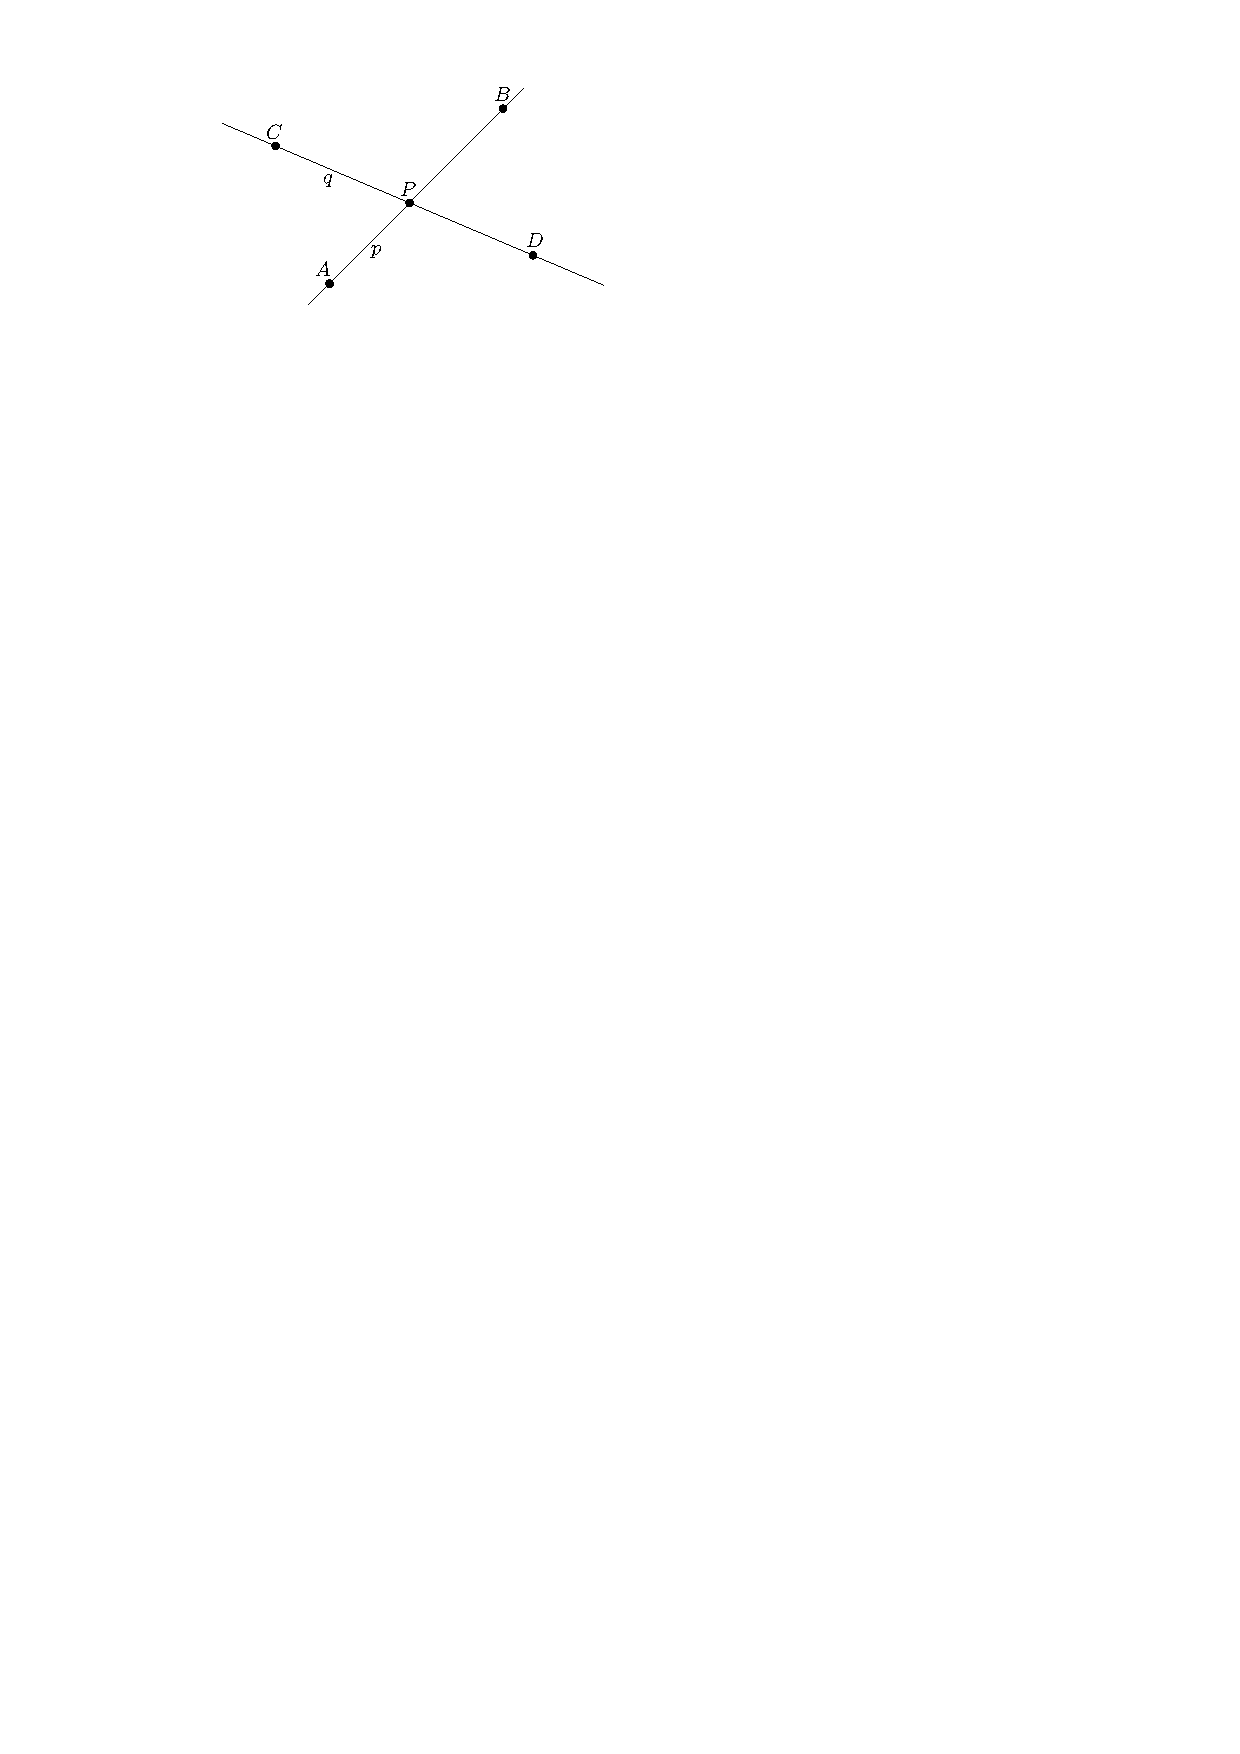
\includegraphics{../img/prusecik.pdf}
	\caption{Průsečík dvou přímek}
	\label{fig:prusecik}
\end{figure}

Průsečík musí ležet na obou přímkách a proto musí splňovat jejich obecné rovnice
$ax+by+c=0$.  Vyjádřeme si nyní obecné rovnice obou přímek. To můžeme
nejjednodušeji udělat pomocí normálových vektorů přímek. Mějme směrové vektory
přímek $p$: $u = (x_2-x_1,y_2-y_1)$ a $q$: $v=(x_4-x_3,y_4-y_3)$ pak normálové
vektory získáme jako $m = (-u_y,u_x)$ a $n = (-v_y,v_x)$. Obecná rovnice přímky
$p$ pak bude $m_xx+m_yy=c$ a přímky $q$ bude $n_xx+n_yy=d$. Koeficienty $c$ a
$d$ získáme dosazením bodů $A$ a $C$ do rovnic: $c = m_xx_1+m_yy_1$,
$d=n_xx_3+n_yy_3$. Pro průsečík musí platit obě rovnice, tedy 
\begin{eqnarray*}
m_xx+m_yy &=& m_xx_1+m_yy_1\\
n_xx+n_yy &=& n_xx_3+n_yy_3
\end{eqnarray*}
Tuto soustavu dvou rovnic o dvou neznámých můžeme řešit například pomocí
determinantů Cramerovým pravidlem $x_i = \frac{|A_i|}{|A|}$:

$$x = \frac{
	\begin{vmatrix}
		c & m_y \\
		d & n_y
	\end{vmatrix}
}
{
	\begin{vmatrix} 
		m_x & m_y \\
		n_x & n_y 
	\end{vmatrix}
}\,\!,\qquad
y = \frac{
	\begin{vmatrix}
		m_x & c \\
		n_x & d
	\end{vmatrix}
}
{
	\begin{vmatrix} 
		m_x & m_y \\
		n_x & n_y 
	\end{vmatrix}
}
$$

Pokud vzorec roznásobíme, získáme pro $x$-ovou souřadnici zlomek:
$$
x=\frac{(x_1 y_2-y_1 x_2)(x_3-x_4)-(x_1-x_2)(x_3 y_4-y_3 x_4)}
{(x_1-x_2)(y_3-y_4)-(y_1-y_2)(x_3-x_4)}$$
Tímto výrazem pak dokážeme jednoduše spočítat průsečík dvou přímek, pokud známe
souřadnice dvou bodů na každé z nich.

\section{Reprezentace čísel}
V~průběhu dalšího zpracování budeme potřebovat počítat průsečíky úseček daných
uzly. Protože průsečíky úseček nebudou mít celočíselné souřadnice, je potřeba
rozmyslet, jakým způsobem je reprezentovat.

{\tuc Čísla s~plovoucí desetinnou čárkou} se pro tyto účely nehodí, protože
nejsou přesná. Při výpočtech s~nimi vznikají zaokrouhlovací chyby, které mohou
zapříčinit špatné pořadí blízkých průsečíků v~uspořádání. Potřebujeme proto
přesnou reprezentaci.

{\tuc Zlomky} jsou pro reprezentaci desetinných čísel vhodnější. Dokážeme pomocí
nich přesně reprezentovat desetinná čísla. Zlomky můžeme vždy
upravit tak, aby jejich jmenovatel byl kladný.  Takové zlomky můžeme porovnávat
podle pravidla $\frac{a}{b} < \frac{c}{d} \Leftrightarrow a\cdot d < c\cdot b $. 
Pokud se nám ale stane, že porovnáváme dva zlomky, které mají vysoký čitatel i
jmenovatel, nemusí nám 64 bitů přesnosti stačit.

Předpokládejme, že máme město velikosti Prahy, což je přibližně $20 \times
30$\,km s~přesností na 10\,cm. O~úsečkách víme, že žádná nebude delší než 300
metrů, tudíž rozdíl jejich souřadnic nebude větší než 3\,000. Pokud budeme
maximalizovat jmenovatele, ze vzorce pro výpočet průsečíku vychází, že můžeme
dosáhnout nejvýše 9 milionů, protože jde o~součin dvou rozdílů souřadnic a každý
bude nejvýše 3\,000.

Tato situace opravdu může nastat, například pro vodorovnou a svislou úsečku
o~délce 300\,m, dotýkající se v~krajním bodě, tzn. $A=(3\,000,0),B=(0,0)$,
$C=(0,3000),D=(0,0)$. Tyto dvě mají průsečík, tudíž se nám mohou při počítání
vyskytnout. Pokud nyní vezmeme téměř totožnou situaci, ale úsečky budou posunuty
směrem k~maximu $x$-ové osy, pak bude $x$-ová souřadnice reprezentovat číslo
30\,km při přesnosti 10\,cm ve zlomku se jmenovatelem 9 milionů. Bude to tedy
číslo $30\cdot1\,000\cdot10\cdot9\cdot10^6=27 \cdot 10^{11}$. Na reprezentaci tohoto
čísla budeme potřebovat $\log_2 27\cdot 10^{11} \doteq 42$ bitů. Pokud tento
zlomek budeme chtít porovnat s~jiným zlomkem s~maximálním jmenovatelem, budeme
potřebovat $42 + \log_2 (9\cdot 10^{6}) \doteq 65$ bitů, na což nám 64bitová proměnná
nebude stačit.

{\tuc Smíšená čísla} nemají ani jednu z~předchozích nevýhod. Jsou to čísla,
která mají tvar $a+\frac{b}{c}$, kde $\frac{b}{c}<1$. Číslo $a$ nazvěme
základem, $b$ čitatelem a $c$ jmenovatelem. U~smíšených čísel je stejně jako
u~zlomků zachována přesnost, ale můžeme je porovnávat bez rizika přetečení.
Pokud se čísla liší v~základu, pak přeteční nehrozí, protože základy se
porovnávají přímo. Pokud mají dvě smíšená čísla stejné základy, pak porovnáme
jejich zlomky. To ale na rozdíl od přímého porovnávání zlomků není problém,
protože jmenovatel je opět nejvýše 24bitový a protože čitatel je nejvýše tak
velký jako jmenovatel, jejich vynásobením vznikne nejvýše 48bitové číslo.
Protože proměnné máme 64bitové, nikde k~přetečení nedojde.

Smíšená čísla jsou implementována jako struktury se členy \verb|base| pro
základ, \verb|numer| pro čitatele a \verb|denom| pro jmenovatele. Všechny
položky jsou 64bitová celá čísla a jmenovatel nesmí být záporný. Pro práci se
smíšenými čísly jsou definovány pomocné funkce v~souboru \verb|mixnum.h|.

\section{Spojky mezi cestami}
\subsection{Příprava dat}
Spojky budeme vytvářet mezi cestami, po kterých budeme posléze vyhledávat.
Nejprve si proto všechny cesty ve funkci \verb|makeGraph| projdeme a roztřídíme
do dvou polí. 

Pole \verb|wayGraph| obsahuje pro každý uzel pole všech jeho sousedů po cestách,
po kterých se bude vyhledávat. Pole \verb|barGraph| obsahuje ty dvojice indexů
uzlů, které spolu sousedí na některé cestě označené jako překážka. Obě pole
reprezentují graf, první pomocí seznamu sousedů, druhé pomocí seznamu hran.
Každé pole budeme využívat jiným způsobem, a proto se nám hodí různá
reprezentace.

Jako druhý krok nalezneme všechny kandidáty na spojky. Zde využijeme mřížky.
Protože spojky chceme dlouhé nejvíce 20 metrů a mřížka má čtverce o~hraně také
20 metrů, stačí nám při hledání možných spojek pro daný bod se podívat pouze na
body ve čtverci, kde sám leží, v~sousedních čtvercích napravo od něj (nahoře,
uprostřed a dole) a ve čtverci pod ním. Protože jsou spojky kratší než 20\,m,
nemohou dále než do sousedního čtverce dosáhnout a protože procházíme postupně
všechny čtverce, možné spojky doleva a nahoru již známe ze zpracování
předchozích čtverců. 

Jednotlivé počáteční a koncové body spojek získáme ze všech bodů v~daném čtverci
vytříděním těch, které mají nějaké sousedy v~poli \verb|wayGraph|. Nepřidáváme
ale všechny spojky, protože pak existovalo např. u kruhových cest v parcích
mnoho spojek, které nepřinášely výrazné zlepšení. Zvolili jsme proto náhodný
výběr, při němž pro každý bod vybereme z každého čtverce mřížky jen několik
kandidátů. Zkoumali jsme vliv počtu kandidátů na délku trasy a jako optitmum se
ukázalo zvolit dva body jako kandidáty z každého čtverce mřížky. Při větším
množství bodů se výslledky zlepšovaly přibližně o procento, ale velikost
výstupního souboru rostla přibližně o šest procent.

%TODO: obrázek

\subsection{Datové struktury}
Když máme připravené kandidáty na spojky a seznam všech překážek, můžeme
přistoupit k~zametání roviny. Zametání roviny probíhá ve funkci
\verb|findDirectWays|. Nejprve popíšeme používané struktury a proměnné.

Struktura \verb|line_t| reprezentuje úsečku v~rovině. Při vytváření se jí
nastavují tyto atributy:
\begin{itemize}
	\item \verb|startlon| a \verb|startlat| udávají souřadnice začátku
	úsečky. Začátek úsečky má vždy nejvýš tak velkou souřadnici $x$, jako
	konec.
	\item \verb|endlon| a \verb|endlat| udávají souřadnice konce úsečky.
	Souřadnice začátků a konců jsou vždy celočíselné, proto je
	reprezentujeme 64bitovými celými čísly.
	\item \verb|startid| a \verb|endid| udávají identifikátor začátku a
	konce úsečky v~OSM.
	\item \verb|isBar| říká, jestli je daná úsečka překážkou.
\end{itemize}
V~průběhu zametání roviny jsou úsečkám nastavovány následující atributy:
\begin{itemize}
	\item \verb|broken| říká, jestli má průsečík s~jinou úsečkou a alespoň
	jedna z~nich je překážka.
	\item \verb|started| udává, že byla zařazena do průřezu.
	\item \verb|ended| udává, že byla v~průžezu a již skončila.
\end{itemize}

Globální pole \verb|lines| s prvky typu \verb|line_t| obsahuje všechny kandidáty
na spojky, globální pole \verb|bars| s prvky typu \verb|line_t| obsahuje všechny
překážky. 

Pro zametání budeme také potřebovat haldu, ze které budeme vybírat nejbližší
událost. V~našem případě používáme haldy dvě, první (\verb|seQueue|), kterou na
začátku naplníme událostmi začátek a konec úsečky, a druhou (\verb|intQueue|),
kterou budeme průběžně plnit průsečíkovými událostmi. V~každém průběhu hlavního
cyklu pak vybereme tu událost, která nastane dříve. Samotné haldy jsou pak
reprezentovány v~poli pomocí binárních hald z~LibUCW. 

Haldy obsahují struktury typu \verb|event_t| respektive \verb|int_event_t| pro
počáteční a koncové respektive průsečíkové události. Struktury mají následující
prvky:
\begin{itemize}
	\item \verb|lon| a \verb|lat| udávají souřadnice události. V~případě
	začátků a konců se jedná o~64bitová celá čísla, v~případě průsečíků se
	jedná o~čísla smíšená. 
	\item \verb|dlon| a \verb|dlat| udávají směrnici úsečky, které se
	událost týká. V~případě průsečíků se jedná o~tu, která by byla
	zpracována dříve.
	\item \verb|lineIdx| je index úsečky, které se událost týká
	\item \verb|line2Idx| se vyskytuje pouze u~průsečíků a jde o~index druhé
	úsečky, které se událost týká.
\end{itemize}


\subsection{Reprezentace průřezu}
Také budeme potřebovat vyhledávací strom, ve kterém si budeme pamatovat aktuální
pořadí úseček v~průřezu. Pro jeho reprezentaci jsme zvolili červeno-černé stromy
z~LibUCW. V~jeho vrcholech jsou uloženy jednotlivé úsečky, které jsou aktuální
pro daný průřez. Protože se ale úsečky mohou křížit, použili jsme několik
vlastních rozšíření. 

Museli jsme si napsat vlastní {\tuc porovnávací funkci}. Zametáme podle $x$-ové
souřadnice tudíž ve stromě potřebujeme mít úsečky seřazené podle $y$-ové
souřadnice v~daném bodě. Ta se ale s~kažým posunutím zametací přímky mění,
proto ve stromě najdeme pouze indexy do pole \verb|lines| na jednotlivé úsečky.
Porovnávací funkce dostane tyto indexy, z~globální proměnné \verb|lon| zjistí,
jaká je aktuální $x$-ová souřadnice zametací přímky, a vypočítá $y$-ovou
souřadnici porovnávaných úseček v~daném bodě. Pokud se $y$-ové souřadnice liší,
pak vrátí výsledek, pokud jsou shodné, porovnávají se podle úhlu. 

K~tomuto je zapotřebí globální proměnná \verb|anglesign|, která říká, s~jakým
znaménkem se má úhel brát. Pokud totiž srovnáváme úsečky při přidávání, zajímá
nás, v~jakém úhlu pokračují dále, naopak při odebírání nás zajímá, pod jakým
úhlem přicházejí. Seřazení je v~tomto případě přesně opačné. Úsečka, která
mířila nejvíce k~severu, tudíž byla na začátku poslední z~daného bodu, bude na
konci přicházet z~jihu, tudíž bude mezi prvními. Úhly úseček nepotřebujeme
počítat, stačí nám porovnat jejich směrnice, což jsou zlomky, a to umíme rychle
a beze ztráty přesnosti.

Ve stromě dále musíme umět prohodit dva sousední vrcholy při průsečíku jim
odpovídajících úseček. Protože si ve vrcholech pamatujeme pouze indexy do pole
úseček, stačí při překřížení tyto indexy prohodit. Struktura stromu i korektnost
uspořádání tím zůstanou zachovány.

Stromy v~LibUCW umí i mazání vrcholu podle pointeru na něj, což se nám hodí při
událostech konec úsečky, protože ji nemusíme hledat, ale stačí si při vytváření
úsečky uložit pointer na vrchol stromu do pole \verb|lineNodes| a při křížení
úseček prohodit patřičné ukazatele. Při mazání se pak jen podíváme podle indexu
úsečky do správného místa v~poli a patřičný vrchol smažeme. Je to výhodou i
v~situaci, kdy nastal při zametání nějaký problém a neproběhla nějaká událost
křížení, a tudíž bychom standardní cestou vrchol nenašli.

Při vkládání nového vrcholu do stromu také potřebujeme zjistit sousedy nově
vloženého vrcholu, abychom přidali případné události křížení. Tuto funkci stromy
v~LibUCW již také obsahují, tudíž nám stačí ji jen využít. Sousedy rovněž
hledáme při křížení, protože překřížením úseček se sousedství změnilo.


\subsection{Zametání}
Události procházíme seřazené nejprve podle délky, pak podle šířky. Pokud jsou
dvě události na stejném místě, nejprve se zpracují události konce úsečky, poté
průsečíky a nakonec události začátku úsečky. Pokud nastane více událostí téhož
typu na stejném místě, zpracovávají se podle úhlu úseček, viz rozbor pořadí ve stromě. 

Dokud máme v~haldě nějaké události, vybereme vždy tu nejbližší a zpracujeme ji.
Pokud se jedná o~začátek úsečky, zkontrolujeme, jestli ve stromě již není, či
zda v~něm není nějaká, se kterou by byla nerozlišitelná. Protože dvě úsečky,
které leží přesně přes sebe jsou nedefinovaný stav, tak tu, která přijde ke
zpracování jako druhá, ignorujeme. Úsečku následně vložíme do průřezového stromu
a zkontrolujeme sousední úsečky, zda se s~nově přidanou nekříží. Pokud ano, tak
přidáme příslušné průsečíkové události do průsečíkové haldy.

Jedná-li se o~konec úsečky, zkontrolujeme, zda úsečka začala (byla přidána do
stromu). Pokud ne, skončíme. Následně zjistíme, zda odstraněním této úsečky se
její sousedé neprotnou, případně přidáme průsečíkovou událost. Nakonec úsečku
smažeme z~průřezového stromu.

Pokud se jedná o~průsečík, nejprve zkontrolujeme, jestli jsme danou událost již
nezpracovali. Pokud se totiž dvě úsečky protínají a během toho, co se k~sobě
přibližují se mezi nimi objeví další úsečka, vznikne průsečíková událost těchto
dvou krajních přímek poprvé při přidání pozdější z~nich a podruhé při konci
vnitřní úsečky, přitom se stále jedná o~stejný průsečík. Protože tyto dvě
průsečíkové události se seřadí hned za sebe a protože se každé dvě úsečky
protnou nejvýše jednou, stačí nám si pamatovat poslední událost a pokud je nová
průsečíková událost se stejnými úsečkami, můžeme ji zahodit.

Dále zkontrolujeme, jestli některá z~úseček již neskončila. Pokud se dvě úsečky
potkávají v~koncovém bodě, pak je zbytečné řešit jejich průsečík. Proto nejprve
vyřešíme konce úseček a pokud máme řešit průsečík s~již skončenou úsečkou,
můžeme ho ignorovat. Následně zjistíme, která z~úseček je nyní horní a která
dolní, a prohodíme odkazy na vrcholy stromu v~poli \verb|lineNodes| a rovněž
prohodíme indexy úseček ve vrcholech stromu. Nakonec zjistíme, zda po prohození
nevznikly nové průsečíky, a případně přidáme průsečíkové události.

Když celý cyklus doběhne, přidáme funkcí \verb|addDirectToMap| do seznamu cest
nově vzniklé spojky a jsme hotovi.


\section{Zkratky přes průchozí prostranství}
Abychom mohli vytvářet zkratky přes průchozí prostranství, potřebujeme nejprve
zjistit, které všechny uzly se vyskytují v~tomto prostranství. Pro samotné
vytváření zkratek pak použijeme obdobný způsob jako při hledání spojek mezi
cestami. 

Nejprve vytvoříme pole všech průchozích prostranství.  K~tomuto účelu
slouží funkce \verb|findWalkAreas|. Procházíme postupně všechny cesty a u~každé
kontrolujeme, jestli se jedná o~průchozí prostranství. Pokud ano, pak vytvoříme
strukturu \verb|walk_area_t| obsahující data o~této ploše: Zjistíme, do jakého
podobélníku mřížky plocha zasahuje, a z~tohoto podobdélníku vybereme ty body,
které jsou uvnitř plochy. Body přidáme do pole \verb|nodeIdxs| a cesty do pole
\verb|ways|. Cesty potom rozdělíme na překážky, jejichž indexy uložíme do
atributu \verb|barIdxs| a vyhledávatelné cesty, které uložíme do atributu
\verb|wayIdxs|. Během rozdělování také odstraňujeme duplicitní cesty. 

Jako další krok připravíme kandidáty na zkratky. Použijeme k tomu funkci
\verb|makeAreaCandidates|. Procházíme postupně dvojice bodů v~dané ploše a
hledáme bližší než 300\,m, které nejsou na společné cestě. Neuvažujeme ovšem
všechny dvojice, ale vybíráme pro každý uzel náhodně z ostatních uzlů, protože
při uvažování všech dvojic vznikalo mnoho cest v podobných místech podobným
směrem. Nalezené dvojice následně přidáme do seznamu kandidátů. Experimentálně
jsme zkoumali vliv průměrného počtu sousedů pro jeden vrchol na délku nalezených
cest přes pražskou Stromovku a Letnou. Jako optimální se ukázalo vybírat pro
každý vrchol průměrně dva sousedy. K dalšímu výrazném zlepšení totiž došlo až
pro pět sousedů, což ale při zlepšení o přibližně 10 procent vedlo ke zvýšení
velikosti grafu o 20 procent, což nám již  přišlo nevýhodné.

Vytvoříme také seznam překážek funkcí \verb|makeAreaBarGraph|. Nejprve přidáme
všechny překážky ze seznamu \verb|barIdxs|, poté přidáme všechny cesty
z~\verb|wayIdxs| a nakonec přidáme obvod plochy. Cesty přidáváme proto, aby
nevnikalo příliš mnoho zkratek, což by vedlo ke zvětšování vyhledávacího grafu.
Takto vzniknou pouz zkratky přes volná prostranství a nebudou křížit cesty.

Když máme kandidáty na zkratky i seznam překážek, můžeme použít již popsané funkce
\verb|findDirectWays| a \verb|addDirectToMap| k~odstranění kandidátů
kolidujících
s~překážkami a cestami a k~přidání výsledných zkratek do mapy. Postup od přípravy
kandidátů až po jejich přidání do mapy zopakujeme pro každou průchozí plochu.

\section{Vytvoření vyhledávacího grafu}
Když již máme všechna data připravená, vytvoříme vyhledávací graf. Nejprve do
něj přidáme všechny vrcholy a hrany. Následně graf projdeme do hloubky a
vybereme tu komponentu, která je největší. Poté v~grafu necháme jen vrcholy a
hrany, které do této komponenty patří, a graf uložíme do souboru
\verb|praha-graph.pbf|. 

\chapter{Výsledky}
\label{ch:vysledky}
Pro zhodnocení výsledků našeho vyhledávače jsme provedli dva druhy testů.
V~rámci prvního jsme porovnávali výsledky našeho vyhledávače s~ostatními veřejně
dostupnými vyhledávači spojení. V~druhém testu jsme na pevně dané trase a času
zkoumali, jaký vliv na nalezené trasy má různé nastavení penalt a rychlostí
chůze. Aplikaci jsme také profilovali, abychom zjistili, v~jakých částech se
tráví nejvíce času a měly by se optimalizovat jako první.

\section{Porovnání s~jinými vyhledávači}
Výsledky našeho vyhledávače jsme porovnávali s~veřejně dostupnými vyhledávači
spojení po Praze: IDOS\footnote{\url{http://idos.cz}},
Mapy.cz\footnote{\url{http://mapy.cz}} a Google
Maps\footnote{\url{http://maps.google.com}}. 

IDOS je nejstarší a nejznámější vyhledávač spojení. Jako jediný z~vyhledávačů
nepodporuje hledání pěších tras, vyhledává pouze v~jízdních řádech, přestupy
mezi zastávkami řeší pomocí tabulky, která obsahuje dvojice zastávek a čas
přesunu mezi nimi. Jako vstup je možné zadat adresu, ale vyhledávač nalezne
pouze nejbližší zastávky podle vzdušné vzdálenosti a hledá z~nich / do nich. 
Na druhou stranu umožňuje široké možnosti nastavení vyhledávání spojů -- volbu
minimálních časů na přestup, typů dopravních prostředků, počtu přestupů, \dots

Mapy.cz a Google Maps jsou původně mapové služby, které do svých vyhledávačů
přidaly možnost vyhledávání kromě pěších cest i spojení MHD. Protože se jedná
primárně o~mapové služby, vyhledávače neumožňují žádné (Mapy.cz) nebo jen velmi
omezené (Google Maps) přizpůsobení. 

Při porovnávání vyhledaných spojení jsme všude nechali výchozí nastavení a náš
vyhledávač jsme nastavili tak, jak si myslíme, že jsou nastaveny ostatní
vyhledávače, aby byly výsledky porovnatelné. Konkrétní nastavení je výchozí
nastavení {\tt config/speeds.yaml} v~příloze. Přestupy nebyly nijak
penalizovány, na zastávce bylo nutné mít aspoň 30\,s čas mezi příchodem /
příjezdem a odjezdem.

Testovali jsme následující trasy, které známe i z~reálného provozu. Jednotlivé
trasy zkoumaly různé aspekty vyhledávačů:
\begin{itemize}
	\item {\em Kolej 17. listopadu -- Přírodovědecká fakulta UK, Albertov}\\ Tato
	cesta je zaměřena na obtížnou dopravní situaci okolo kolejí 17.
	listopadu. Spojení na Nádraží Holešovice je nejspolehlivější pěšky,
	autobus 201 většinou nejede dle jízdního řádu. V~případě cesty tramvají
	č. 17 je možné jednak využít od kolejí autobus 112, ovšem s~výstupem na
	Povltavské, nikoli na Trojské, případně dojít přímo na Trojskou pěšky.
	Všechny tyto možnosti dávají smysl při hledání cesty na Albertov. Na
	durhém konci také není situace přímočará, při cestě od metra je dobrou
	alternativou jít pěšky z~Vyšehradu. 
	\item {\em Kolej 17. listopadu -- Čistírna odpadních vod, Bubeneč}\\ Tato
	cesta zkoumá schopnosti pěší navigace, protože jednou z~možností je jít
	pěšky přes Stromovku. Také je zde vidět rozdíl mezi naším vyhledávačem a
	Google Maps na jedné straně a IDOSem a Mapy.cz na straně druhé, které
	využívají znalosti jízdních řádů integrovaných vlaků a umí je na této
	cestě využít.
	\item {\em Kovanecká -- Gymnázium Omská}\\ Tato cesta opět zkoumá schopnost
	využívat delší pěší přesuny a také dávat přednost časově kratším cestám
	s~přestupy. 
	\item {\em FEL ČVUT, Dejvice -- Hlávkova kolej}\\ Tato cesta je zaměřena na
	hledání aktuálně nejrychlejší alternativy z~několika rovnocenných. Dobré
	alternativy nevyžadují dlouhé pěší přesuny.
\end{itemize}
\subsection{Kolej 17.\,listopadu -- Albertov}

Náš vyhledávač našel následující spojení:
\begin{itemize}
\item Spojení 0:\\[0mm]
\vspace*{-0.5cm}
\begin{center}
\begin{tabular}{|c c c r|}\hline
{\bf Zastávka}&{\bf Příjezd}&{\bf Odjezd}&{\bf Linka}\\\hline
Kuchyňka&&13:25&201\\
Nádraží Holešovice&13:28&13:32&C\\
I. P. Pavlova&13:40&&\\\hline
\end{tabular} \\[0mm]
\end{center}
Očekávaný příchod je 13:56.

\item Spojení 2:\\
\vspace*{-0.5cm}
\begin{center}
\begin{tabular}{|c c c r|}\hline
{\bf Zastávka}&{\bf Příjezd}&{\bf Odjezd}&{\bf Linka}\\\hline
Kuchyňka&&13:25&201\\
Nádraží Holešovice&13:28&13:32&C\\
Florenc&13:36&13:41&B\\
Karlovo náměstí&13:46&&\\
Palackého náměstí&&13:52&18\\
Albertov&13:56&&\\\hline
\end{tabular} \\[0mm]
\end{center}
Očekávaný příchod je 14:00.

\item Spojení 3:\\
\vspace*{-0.5cm}
\begin{center}
\begin{tabular}{|l c c r|}\hline
{\bf Zastávka}&{\bf Příjezd}&{\bf Odjezd}&{\bf Linka}\\\hline
Kuchyňka&&13:25&201\\
Nádraží Holešovice&13:28&13:31&6\\
Masarykovo nádraží&13:43&13:44&14\\
Albertov&13:59&&\\\hline
\end{tabular}\\[2mm]
\end{center}
Očekávaný příchod je 14:03.
\end{itemize}

Vyhledávač IDOS našel následující spojení:\\
\vspace*{-0.5cm}
\begin{center}
\begin{tabular}{|l c c r|}\hline
{\bf Zastávka}&{\bf Příjezd}&{\bf Odjezd}&{\bf Linka}\\\hline
Kuchyňka&&13:23&201\\
Bulovka&13:26&13:28&24\\
Albertov&14:04&&\\\hline
\end{tabular}\\
\end{center}
\begin{center}
\begin{tabular}{|l c c r|}\hline
{\bf Zastávka}&{\bf Příjezd}&{\bf Odjezd}&{\bf Linka}\\\hline
Kuchyňka&&13:25&201\\
Nádraží Holešovice&13:28&13:32&C\\
Florenc&13:36&13:41&B\\
Karlovo náměstí&13:47&&\\
Palackého náměstí&&13:52&18\\
Albertov&13:56&&\\\hline
\end{tabular} 
\end{center}

V~tomto spojení se ukázala výhoda vyhledávačů, které umí delší pěší přesuny.
Vlivem výluky není možné jet přímo z~Karlova náměstí na Albertov a nejkratší
cesta se ukazuje být přes I. P. Pavlova. Náš vyhledávač našel tuto trasu ve
stejné podobě jako Google Maps, Mapy.cz ještě využily autobusu 148 k~přiblížení
se. Odhadované časy se liší jen o~rychlost chůze. IDOS kvůli absenci mapových
podkladů nalezl jen trasy vedoucí na Albertov, které náš vyhledávač nalezl také,
i když s~mírně jiným průběhem. 

\begin{center}
\begin{tabular}{|l c c r|}\hline
{\bf Zastávka}&{\bf Příjezd}&{\bf Odjezd}&{\bf Linka}\\\hline
Pelc Tyrolka&&13:26&112\\
Trojská&13:29&13:33&17\\
Výtoň&13:54&13:57&14\\
Albertov&13:59&&\\\hline
\end{tabular} 
\end{center}
\begin{figure}[h]
  \centering
    \includegraphics[height=0.98\textheight]{../img/kolej-albertov-standard.pdf}
  \caption{Spojení Kolej 17. listopadu -- Albertov podle našeho vyhledávače}
  \label{fig:kolej-albertov-standard}
\end{figure}
\begin{figure}[h]
  \centering
    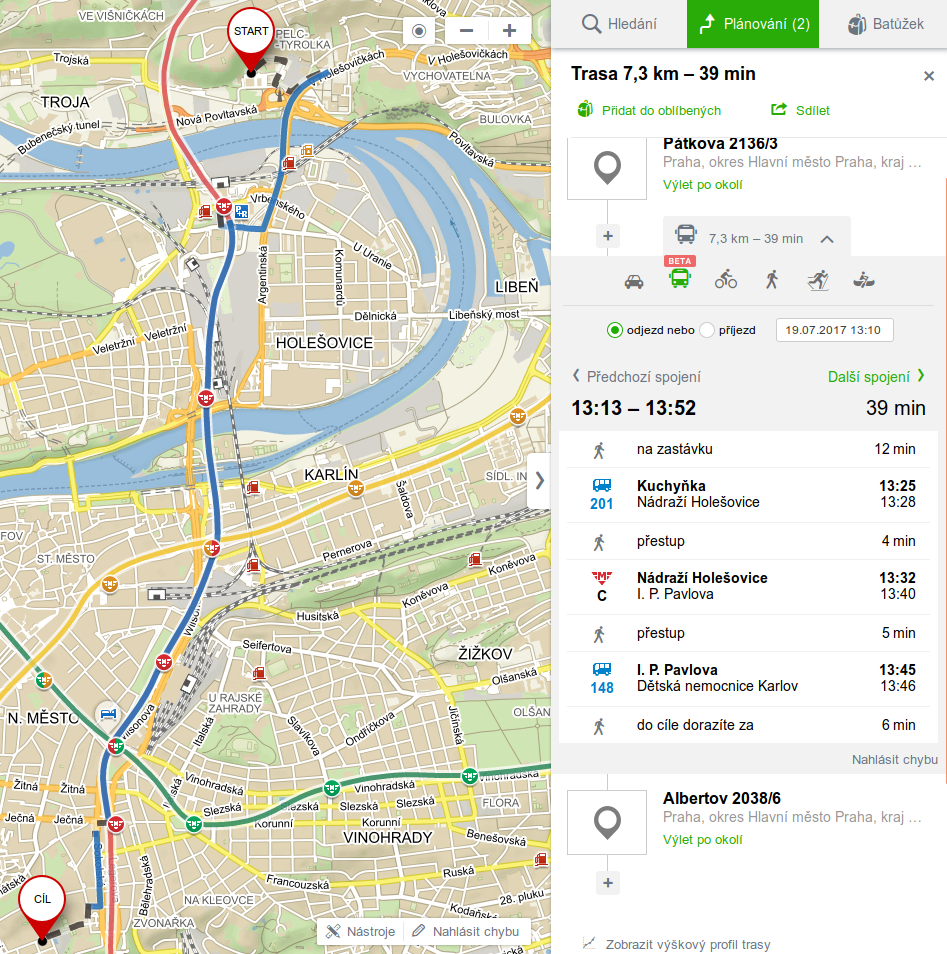
\includegraphics[width=\textwidth]{../img/kolej-albertov-seznam.png}
  \caption{Spojení Kolej 17. listopadu -- Albertov podle Mapy.cz}
  \label{fig:kolej-albertov-seznam}
\end{figure}
\begin{figure}[h]
  \centering
    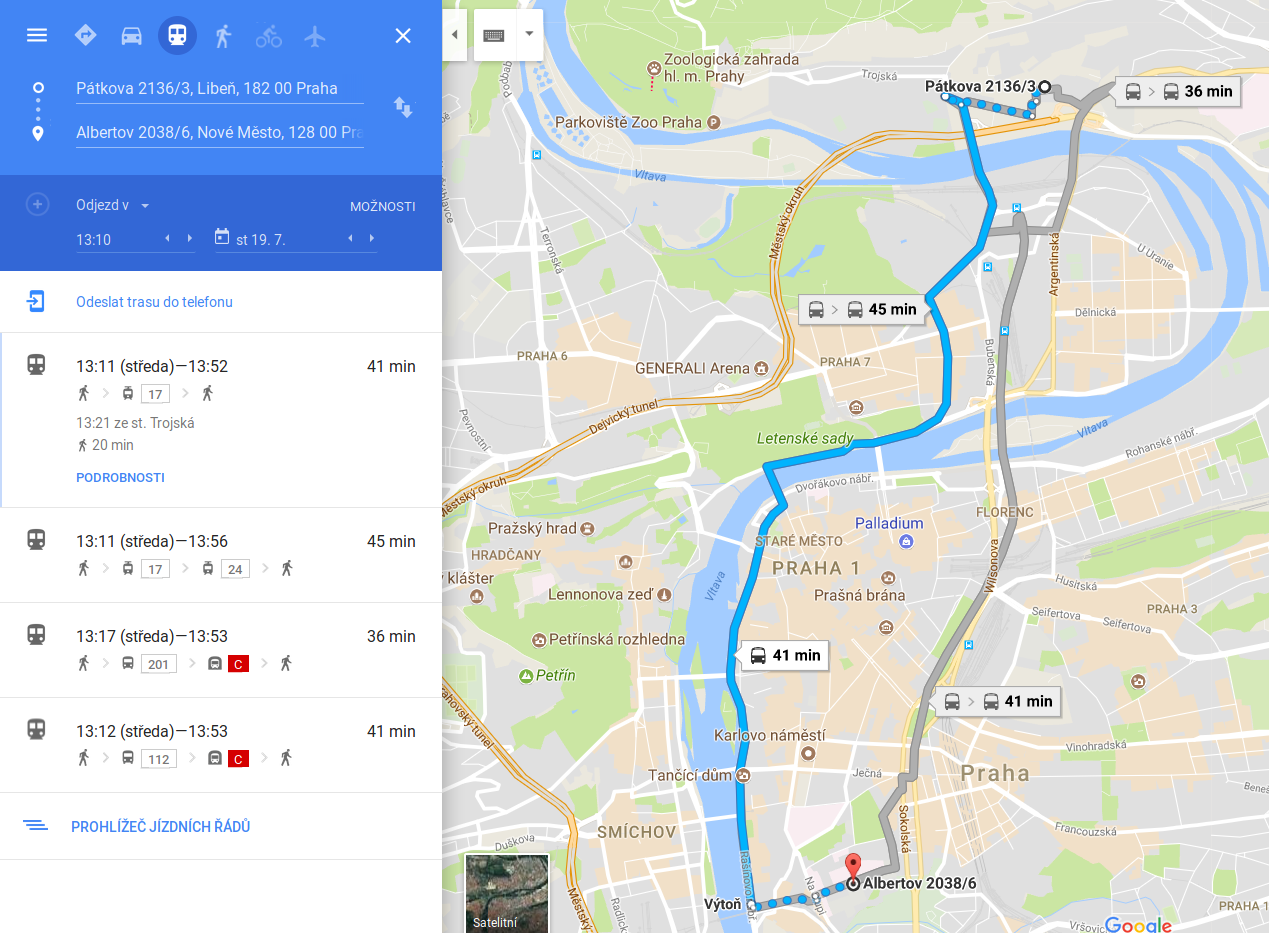
\includegraphics[width=\textwidth]{../img/kolej-albertov-google.png}
  \caption{Spojení Kolej 17. listopadu -- Albertov podle Google Maps}
  \label{fig:kolej-albertov-google}
\end{figure}

\clearpage
\subsection{Kolej 17.\,listopadu -- Čistírna odpadních vod}

Spojení 0 nevyžaduje žádný přesun pomocí MHD, celá trasa je vedena pěšky.
Očekávaný příchod je 14:08.

\begin{itemize}
\item Spojení 1:\\
\vspace*{-0.5cm}
\begin{center}
\begin{tabular}{|l c c r|}\hline
{\bf Zastávka}&{\bf Příjezd}&{\bf Odjezd}&{\bf Linka}\\\hline
Kuchyňka&&13:25&201\\
Nádraží Holešovice&13:28&13:31&6\\
Strossmayerovo náměstí&13:36&13:39&26\\
Hradčanská&13:47&14:00&131\\
Goeteho&14:03&&\\\hline
\end{tabular}\\[2mm]
\end{center}
Očekávaný příchod je 14:08.

\item Spojení 4:\\
\vspace*{-0.5cm}
\begin{center}
\begin{tabular}{|l c c r|}\hline
{\bf Zastávka}&{\bf Příjezd}&{\bf Odjezd}&{\bf Linka}\\\hline
Kuchyňka&&13:25&201\\
Nádraží Holešovice&13:28&13:31&6\\
Strossmayerovo náměstí&13:36&13:39&26\\
Vítězné náměstí&13:50&&\\
Dejvická&&13:55&160\\
Nádraží Podbaba&13:59&&\\\hline
\end{tabular}\\[2mm]
\end{center}
Očekávaný příchod je 14:09. 

\item Spojení 6:\\
\vspace*{-0.5cm}
\begin{center}
\begin{tabular}{|l c c r|}\hline
{\bf Zastávka}&{\bf Příjezd}&{\bf Odjezd}&{\bf Linka}\\\hline
Kuchyňka&&13:25&201\\
Nádraží Holešovice&13:28&13:31&6\\
Dlouhá třída&13:38&13:42&8\\
Nádraží Podbaba&14:02&&\\\hline
\end{tabular}\\[2mm]
\end{center}
Očekávaný příchod je 14:12. 

\end{itemize}

Vyhledávač IDOS našel následující spojení:\\
\vspace*{-0.5cm}
\begin{center}
\begin{tabular}{|l c c r|}\hline
{\bf Zastávka}&{\bf Příjezd}&{\bf Odjezd}&{\bf Linka}\\\hline
Kuchyňka&&13:25&201\\
Nádraží Holešovice&13:28&13:45&Os 10440\\
Praha-Podbaba&13:49&&\\\hline
\end{tabular}\\
\end{center}
\begin{center}
\begin{tabular}{|l c c r|}\hline
{\bf Zastávka}&{\bf Příjezd}&{\bf Odjezd}&{\bf Linka}\\\hline
Pelc Tyrolka&&13:26&112\\
Trojská&13:29&13:33&17\\
Nádraží Holešovice&13:35&13:45&Os 10440\\
Praha-Podbaba&13:49&&\\\hline
\end{tabular} 
\end{center}

Na výsledcích tohoto spojení se významně projevila integrace železničních
jízdních řádů do vyhledávačů. IDOS i Mapy.cz jízdní řády integrované mají,
proto využily vlak mezi stanicemi Praha-Holešovice a Praha-Podbaba. Google Maps
ani náš vyhledávač železniční jízdní řády integrované nemají, nalezly proto
cesty oklikou a s~delšími pěšími přesuny. Náš vyhledávač nalezl obě varianty
cesty bez vlaků, a to přímo pěšky a oklikou přes Letnou, pro přímou cestu při
tomto hledání nevyužil autobus 112 a proto je očekávaný čas horší než u~Google
Maps. Jak se také ukáže u~dalších spojení, odhad rychlosti chůze byl při našem
nastavení o~něco konzervativnější než u~Google Maps, vzálenější pěší přesuny
tudíž vycházejí o~něco delší.


\begin{figure}[h]
  \centering
    \includegraphics[width=\textwidth]{../img/kolej-bubenec-osmawalk.pdf}
  \caption{Spojení Kolej 17. listopadu -- Čistírna odpadních vod podle našeho
  vyhledávače}
  \label{fig:kolej-bubenec-osmawalk}
\end{figure}
\begin{figure}[h]
  \centering
    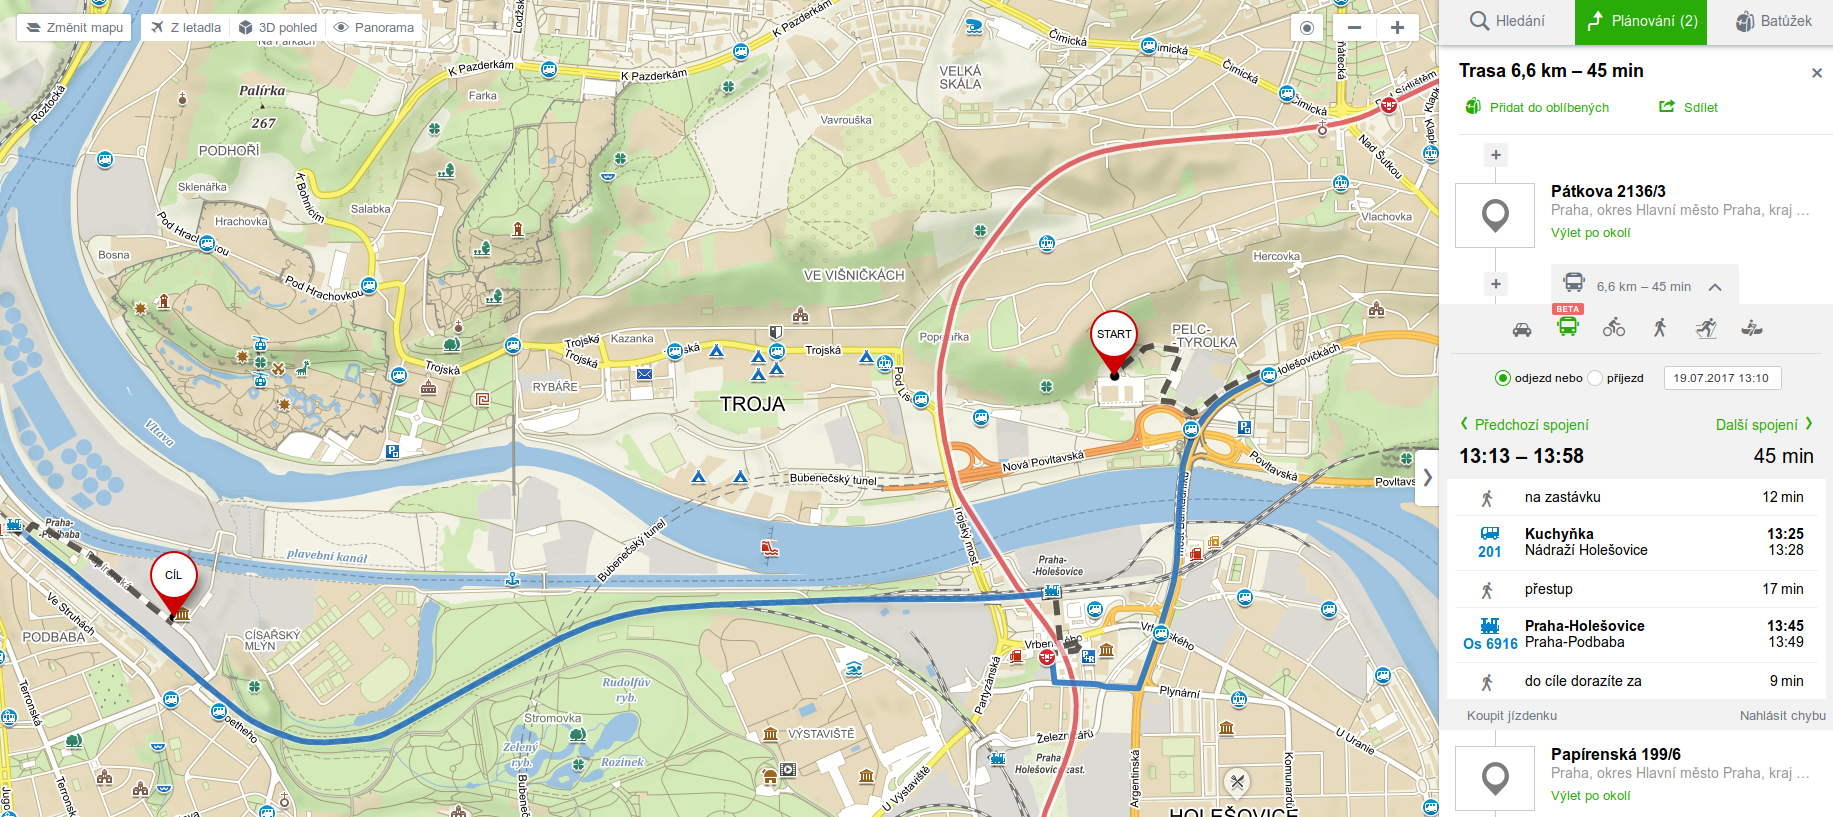
\includegraphics[width=\textwidth]{../img/kolej-bubenec-seznam.png}
  \caption{Spojení Kolej 17. listopadu -- Čistírna odpadních vod podle Mapy.cz}
  \label{fig:kolej-bubenec-seznam}
\end{figure}
\begin{figure}[h]
  \centering
    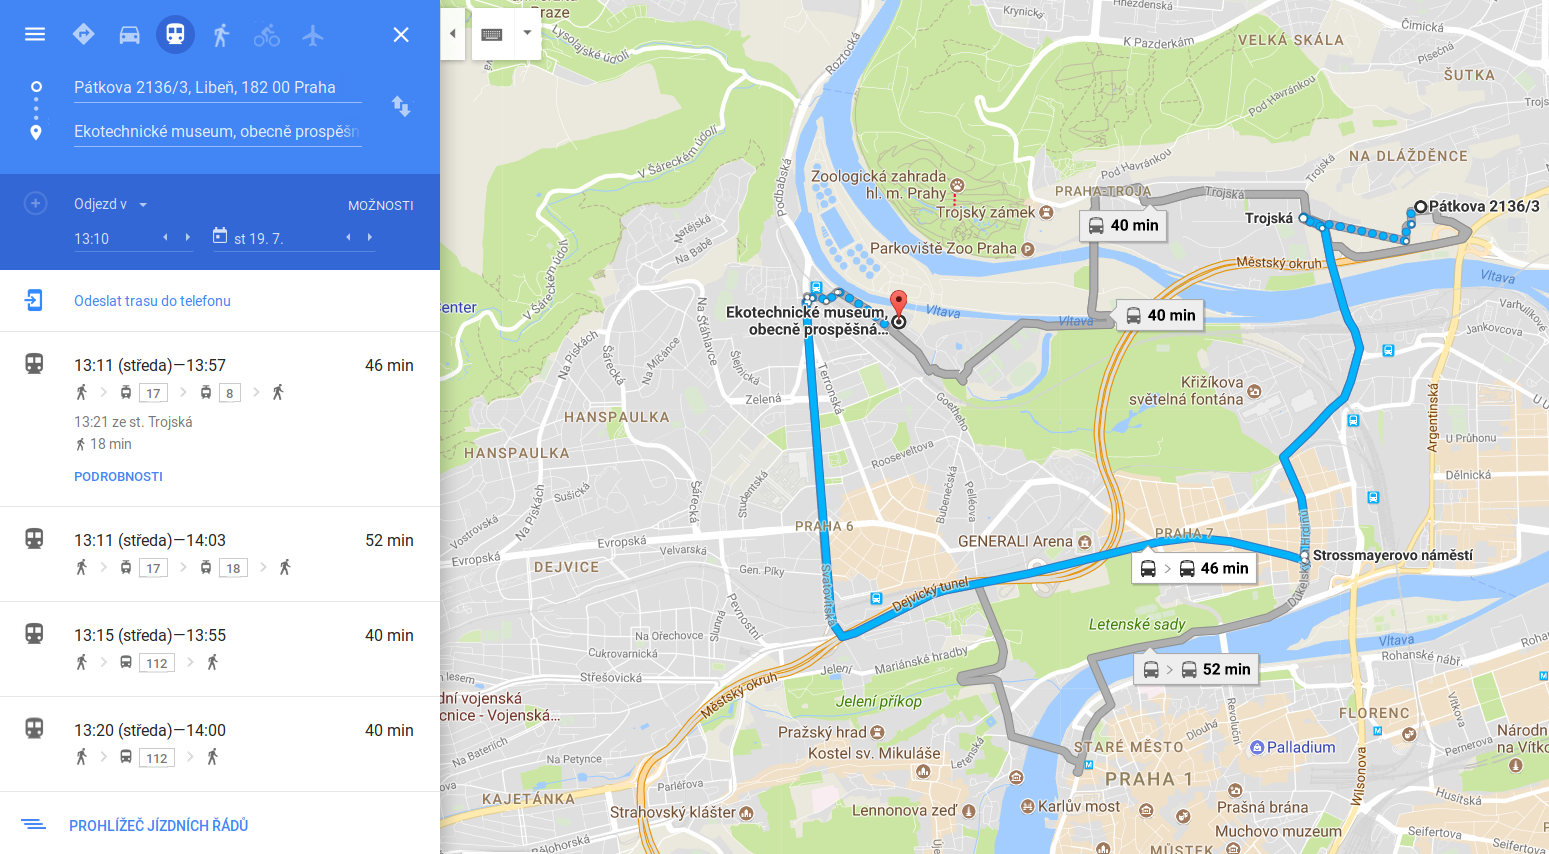
\includegraphics[width=\textwidth]{../img/kolej-bubenec-google.png}
  \caption{Spojení Kolej 17. listopadu -- Čistírna odpadních vod podle Google
  Maps}
  \label{fig:kolej-bubenec-google}
\end{figure}

\clearpage
\subsection{Kovanecká -- Gymnázium Omská}
\begin{itemize}
\item Spojení 0:\\
\vspace*{-0.5cm}
\begin{center}
\begin{tabular}{|l c c r|}\hline
{\bf Zastávka}&{\bf Příjezd}&{\bf Odjezd}&{\bf Linka}\\\hline
Divadlo Gong&&13:21&16\\
Orionka&13:39&13:41&136\\
Bělocerkevská&13:47&&\\\hline
\end{tabular}\\[2mm]
\end{center}
Očekávaný příchod je 13:55.
 
\item Spojení 1:\\
\vspace*{-0.5cm}
\begin{center}
\begin{tabular}{|l c c r|}\hline
{\bf Zastávka}&{\bf Příjezd}&{\bf Odjezd}&{\bf Linka}\\\hline
Divadlo Gong&&13:21&16\\
Mezi hřbitovy&13:32&13:36&26\\
Nad Primaskou&13:42&13:43&7\\
Slavia&13:49&13:52&22\\
Kubánské náměstí&13:53&&\\\hline
\end{tabular}\\[2mm]
\end{center}
Očekávaný příchod je 13:55.
 

\item Spojení 3:\\
\vspace*{-0.5cm}
\begin{center}
\begin{tabular}{|l c c r|}\hline
{\bf Zastávka}&{\bf Příjezd}&{\bf Odjezd}&{\bf Linka}\\\hline
Balabenka&&13:19&25\\
Palmovka&13:21&13:23&24\\
Karlovo náměstí&13:45&13:46&22\\
Kubánské náměstí&14:05&&\\\hline
\end{tabular}\\[2mm]
\end{center}
Očekávaný příchod je 14:07.
 
\item Spojení 5:\\
\vspace*{-0.5cm}
\begin{center}
\begin{tabular}{|l c c r|}\hline
{\bf Zastávka}&{\bf Příjezd}&{\bf Odjezd}&{\bf Linka}\\\hline
Balabenka&&13:19&25\\
Palmovka&13:21&13:23&24\\
Kubánské náměstí&14:06&&\\\hline
\end{tabular}\\[2mm]
\end{center}
Očekávaný příchod je 14:08.
 
\item Spojení 7:\\
\vspace*{-0.5cm}
\begin{center}
\begin{tabular}{|l c c r|}\hline
{\bf Zastávka}&{\bf Příjezd}&{\bf Odjezd}&{\bf Linka}\\\hline
Ocelářská&&13:19&6\\
Kubánské náměstí&14:11&&\\\hline
\end{tabular}\\[2mm]
\end{center}
Očekávaný příchod je 14:13. 
\end{itemize}

Vyhledávač IDOS našel tato spojení:\\
\vspace*{-0.5cm}
\begin{center}
\begin{tabular}{|l c c r|}\hline
{\bf Zastávka}&{\bf Příjezd}&{\bf Odjezd}&{\bf Linka}\\\hline
Balabenka&&13:20&6\\
Kubánské náměstí&14:11&&\\\hline
\end{tabular} \\[2mm]
\end{center}
\begin{center}
\begin{tabular}{|l c c r|}\hline
{\bf Zastávka}&{\bf Příjezd}&{\bf Odjezd}&{\bf Linka}\\\hline
Divadlo Gong&&13:21&16\\
Želivského&13:35&13:41&150\\
Slavia&13:46&13:52&22\\
Kubánské náměstí&13:53&&\\\hline
\end{tabular} 
\end{center}

V~tomto spojení se opět projevila výhoda vyhledávačů, které mají mapové
podklady, protože v~dané relaci je dle zkušeností výhodné nesnažit se dojet co
nejblíže, ale jít pěšky už ze Želivského a projít skrz vinohradskou nemocnici.
Mapy.cz zde daly přednost jízdě bez přestupů, ale bohužel zvolily špatnou
tramvaj, protože linka č. 6 objíždí celé město a cesta jí proto trvá neúměrně
dlouho. IDOS hledal spojení na Kubánské náměstí, což se pro vhodnou volbu
přestupů ukázalo jako poměrně dobrá volba. Google Maps našly cestu skrz
vinohradskou nemocnici, náš vyhledávač místo toho zvolil cestu přes Orionku
která byla jen o~něco delší. Alternativní spojení byly zajímavé jak u~Google
Maps, kde spojení vedlo dokonce až přes Anděl, tak i u~našeho
vyhledávače, který přejel zastávku Kubánské náměstí, aby se pak do ní vrátil
z~druhé strany. Zkoumali jsme, jestli to nemůže být zapříčiněno chybou v~datech,
ale připojení zastávky k~cestní síti se jevilo v~pořádku. 
\begin{figure}[h]
  \centering
    \includegraphics[width=\textwidth]{../img/kovanecka-omska-osmawalk.pdf}
  \caption{Spojení Kovanecká -- Gymnázium Omská podle našeho vyhledávače}
  \label{fig:kovanecka-omska-osmawalk}
\end{figure}
\begin{figure}[h]
  \centering
    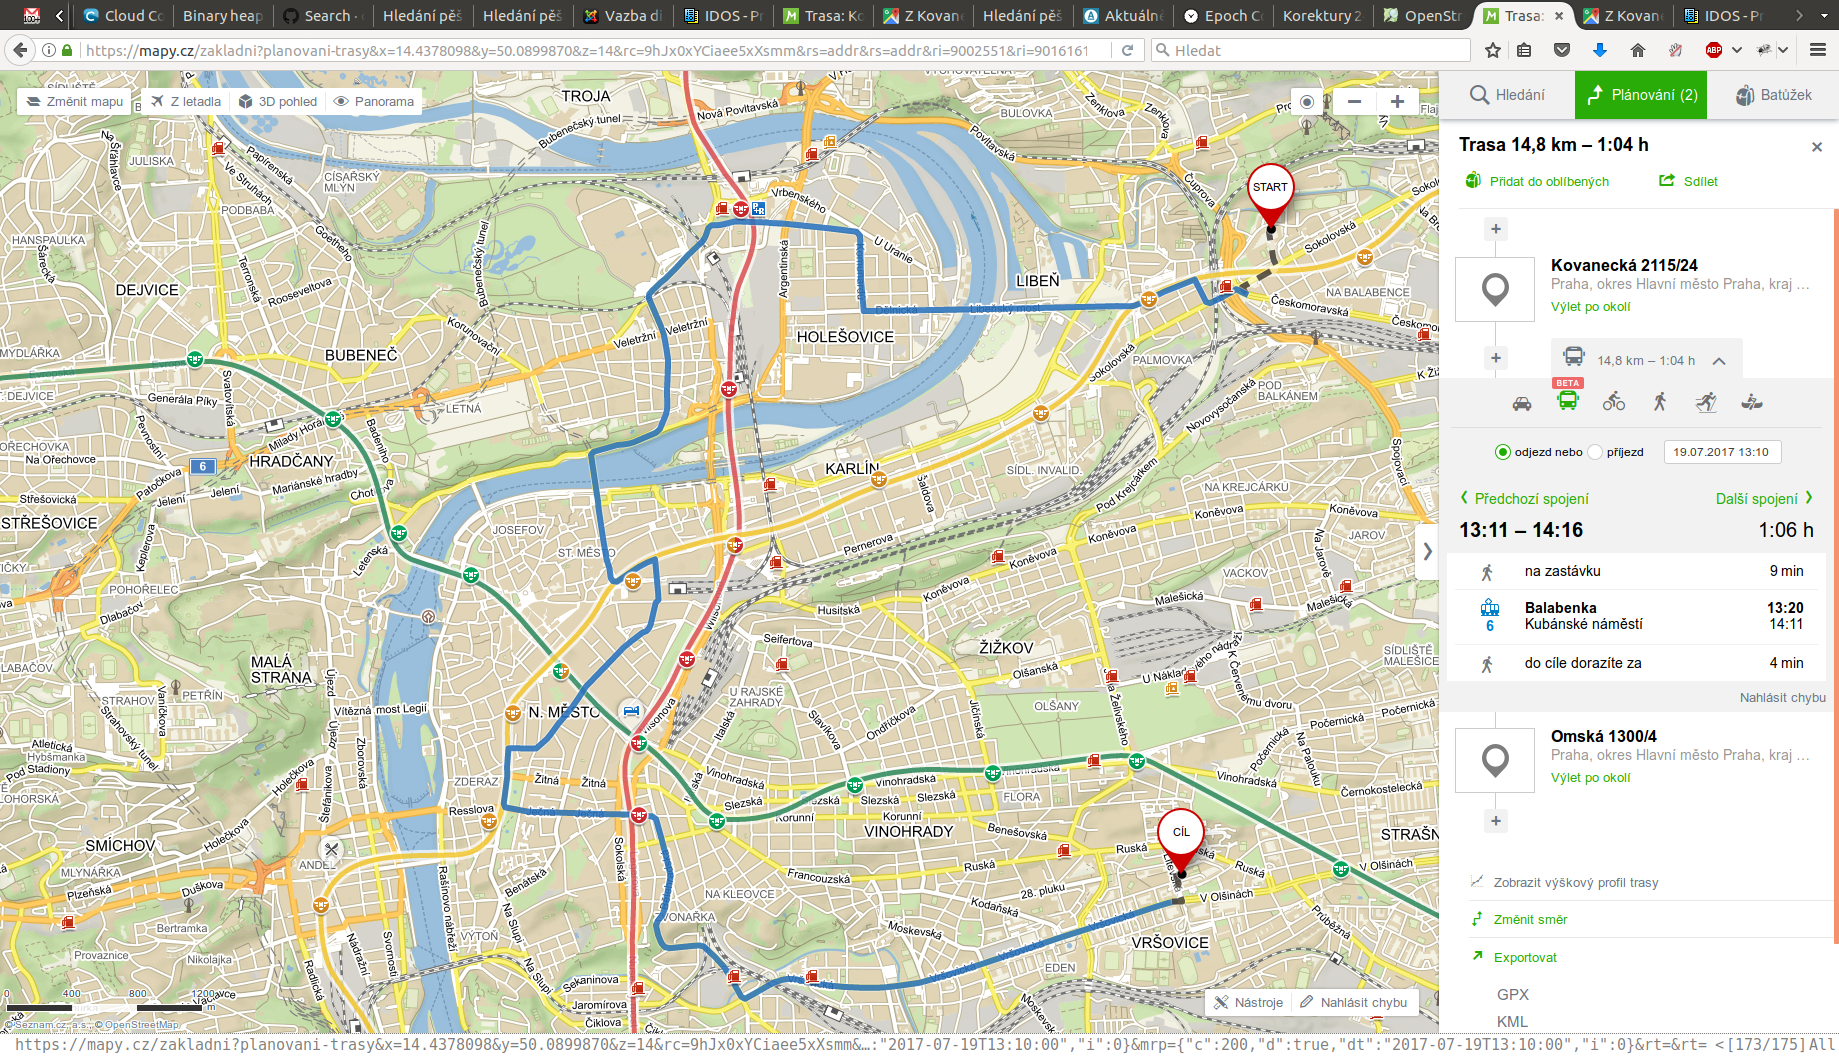
\includegraphics[width=\textwidth]{../img/kovanecka-omska-seznam.png}
  \caption{Spojení Kovanecká -- Gymnázium Omská podle Mapy.cz}
  \label{fig:kovanecka-omska-seznam}
\end{figure}
\begin{figure}[h]
  \centering
    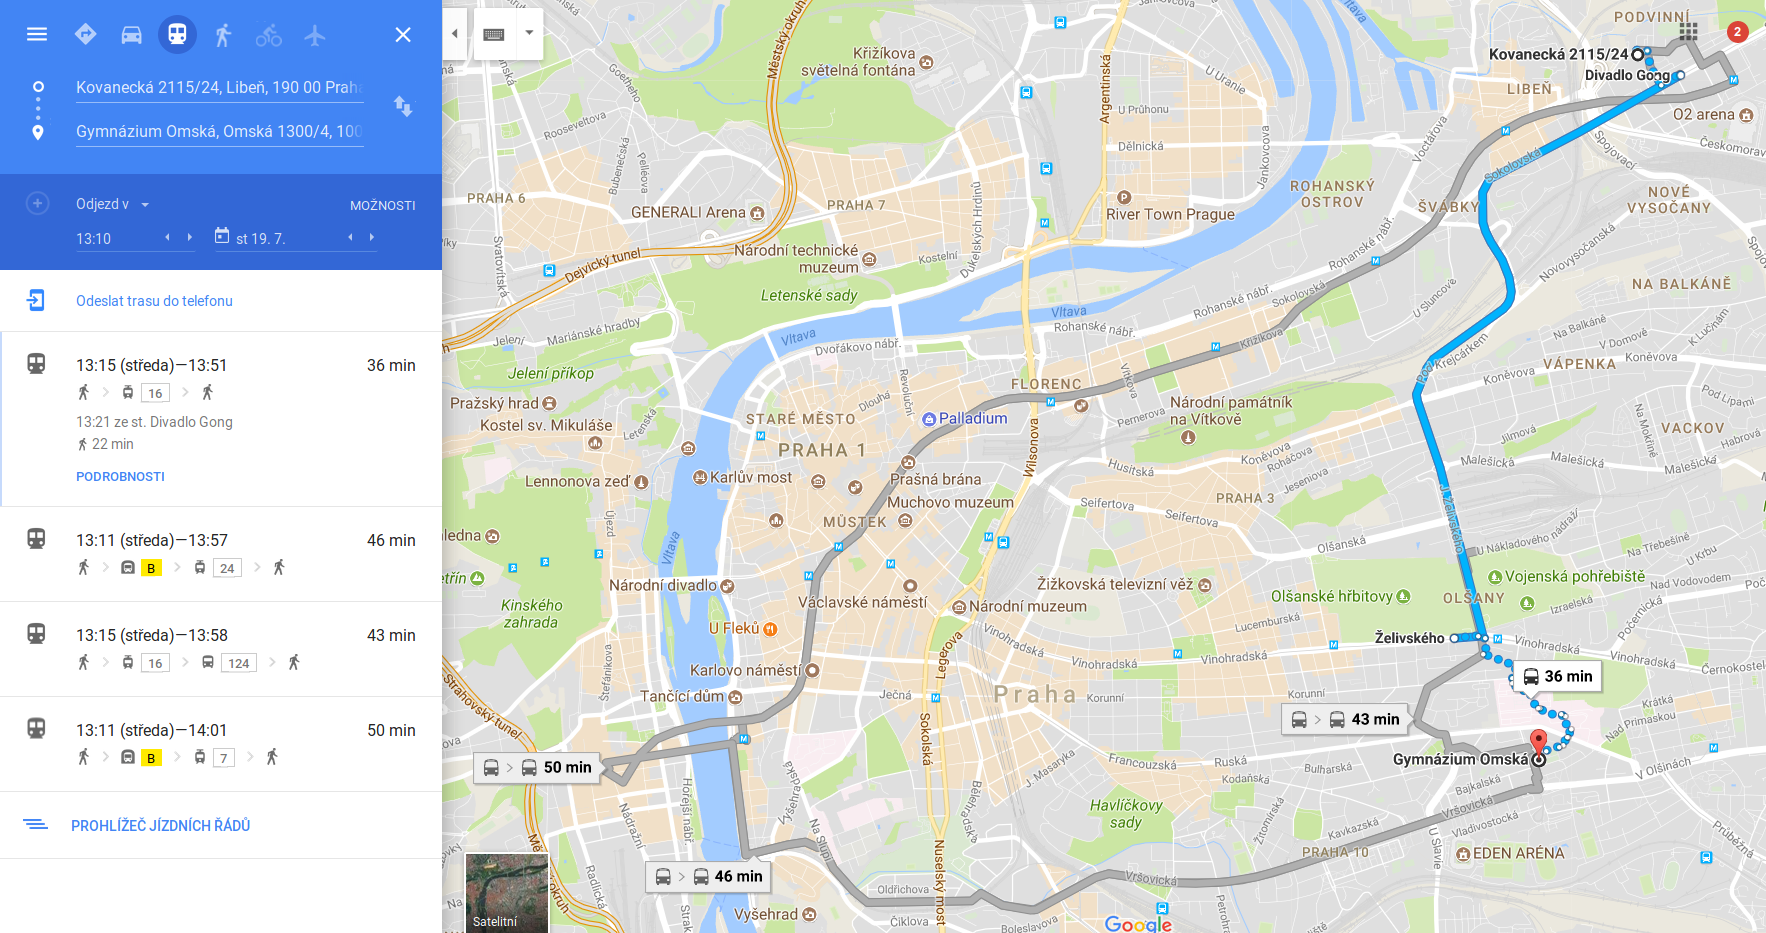
\includegraphics[width=\textwidth]{../img/kovanecka-omska-google.png}
  \caption{Spojení Kovanecká -- Gymnázium Omská podle Google Maps}
  \label{fig:kovanecka-omska-google}
\end{figure}

\clearpage
\subsection{FEL ČVUT -- Hlávkova kolej}
\begin{itemize}
\item Spojení 0:\\
\vspace*{-0.5cm}
\begin{center}
\begin{tabular}{|l c c r|}\hline
{\bf Zastávka}&{\bf Příjezd}&{\bf Odjezd}&{\bf Linka}\\\hline
Dejvická&&13:16&A\\
Malostranská&13:19&13:23&2\\
Moráň&13:34&&\\\hline
\end{tabular}\\[2mm]
\end{center}
Očekávaný příchod je 13:38.

\item Spojení 1:\\
\vspace*{-0.5cm}
\begin{center}
\begin{tabular}{|l c c r|}\hline
{\bf Zastávka}&{\bf Příjezd}&{\bf Odjezd}&{\bf Linka}\\\hline
Lotyšská&&13:18&18\\
Moráň&13:38&&\\\hline
\end{tabular}\\[2mm]
\end{center}
Očekávaný příchod je 13:42.
\end{itemize}


Vyhledávač IDOS našel tato spojení:\\
\vspace*{-0.5cm}
\begin{center}
\begin{tabular}{|l c c r|}\hline
{\bf Zastávka}&{\bf Příjezd}&{\bf Odjezd}&{\bf Linka}\\\hline
Dejvická&&13:16&A\\
Můstek&13:22&13:29&B\\
Karlovo náměstí&13:32&&\\\hline
\end{tabular}\\[2mm]
\end{center}
\begin{center}
\begin{tabular}{|l c c r|}\hline
{\bf Zastávka}&{\bf Příjezd}&{\bf Odjezd}&{\bf Linka}\\\hline
Vítězné náměstí&&13:19&18\\
Karlovo náměstí&13:37&&\\\hline
\end{tabular}\\[2mm]
\begin{tabular}{|l c c r|}\hline
{\bf Zastávka}&{\bf Příjezd}&{\bf Odjezd}&{\bf Linka}\\\hline
Dejvická&&13:21&A\\
Staroměstská&13:25&13:30&18\\
Karlovo náměstí&13:37&&\\\hline
\end{tabular} 
\end{center}

Toto spojení reprezentovalo situaci, kdy samotná trasa je jednoduchá, ale je
množství různých alternativ v~koncových a výchozích stanicích. Náš vyhledávač
našel spojení identická s~Google Maps. Mapy.cz a IDOS nalezly mírně odlišná
spojení využívající i linku metra B, ale časově odpovídající našemu nalezenému
spojení. 

\begin{figure}[h]
  \centering
    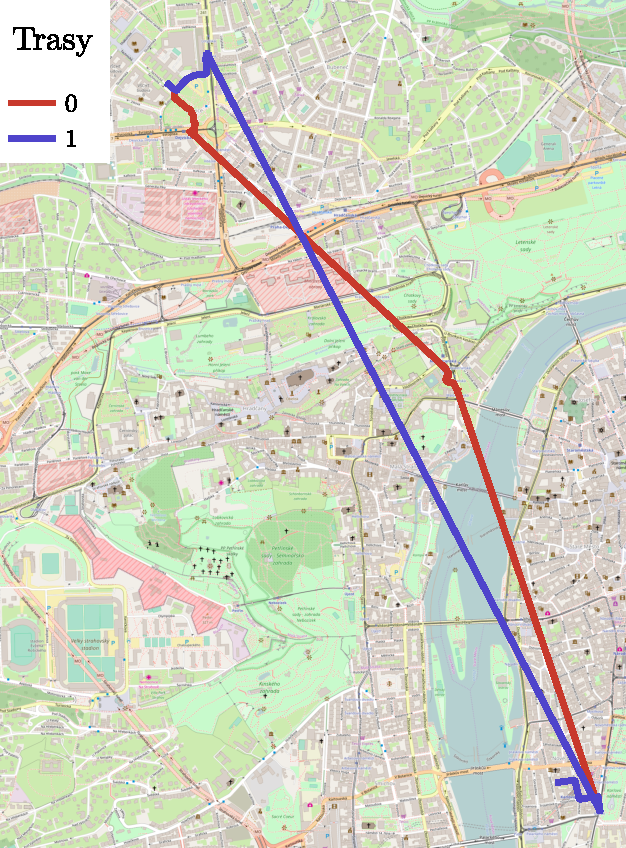
\includegraphics[width=\textwidth]{../img/fel-hlavkova-osmawalk.pdf}
  \caption{Spojení FEL ČVUT -- Hlávkova kolej podle našeho vyhledávače}
  \label{fig:fel-hlavkova-osmawalk}
\end{figure}
\begin{figure}[h]
  \centering
    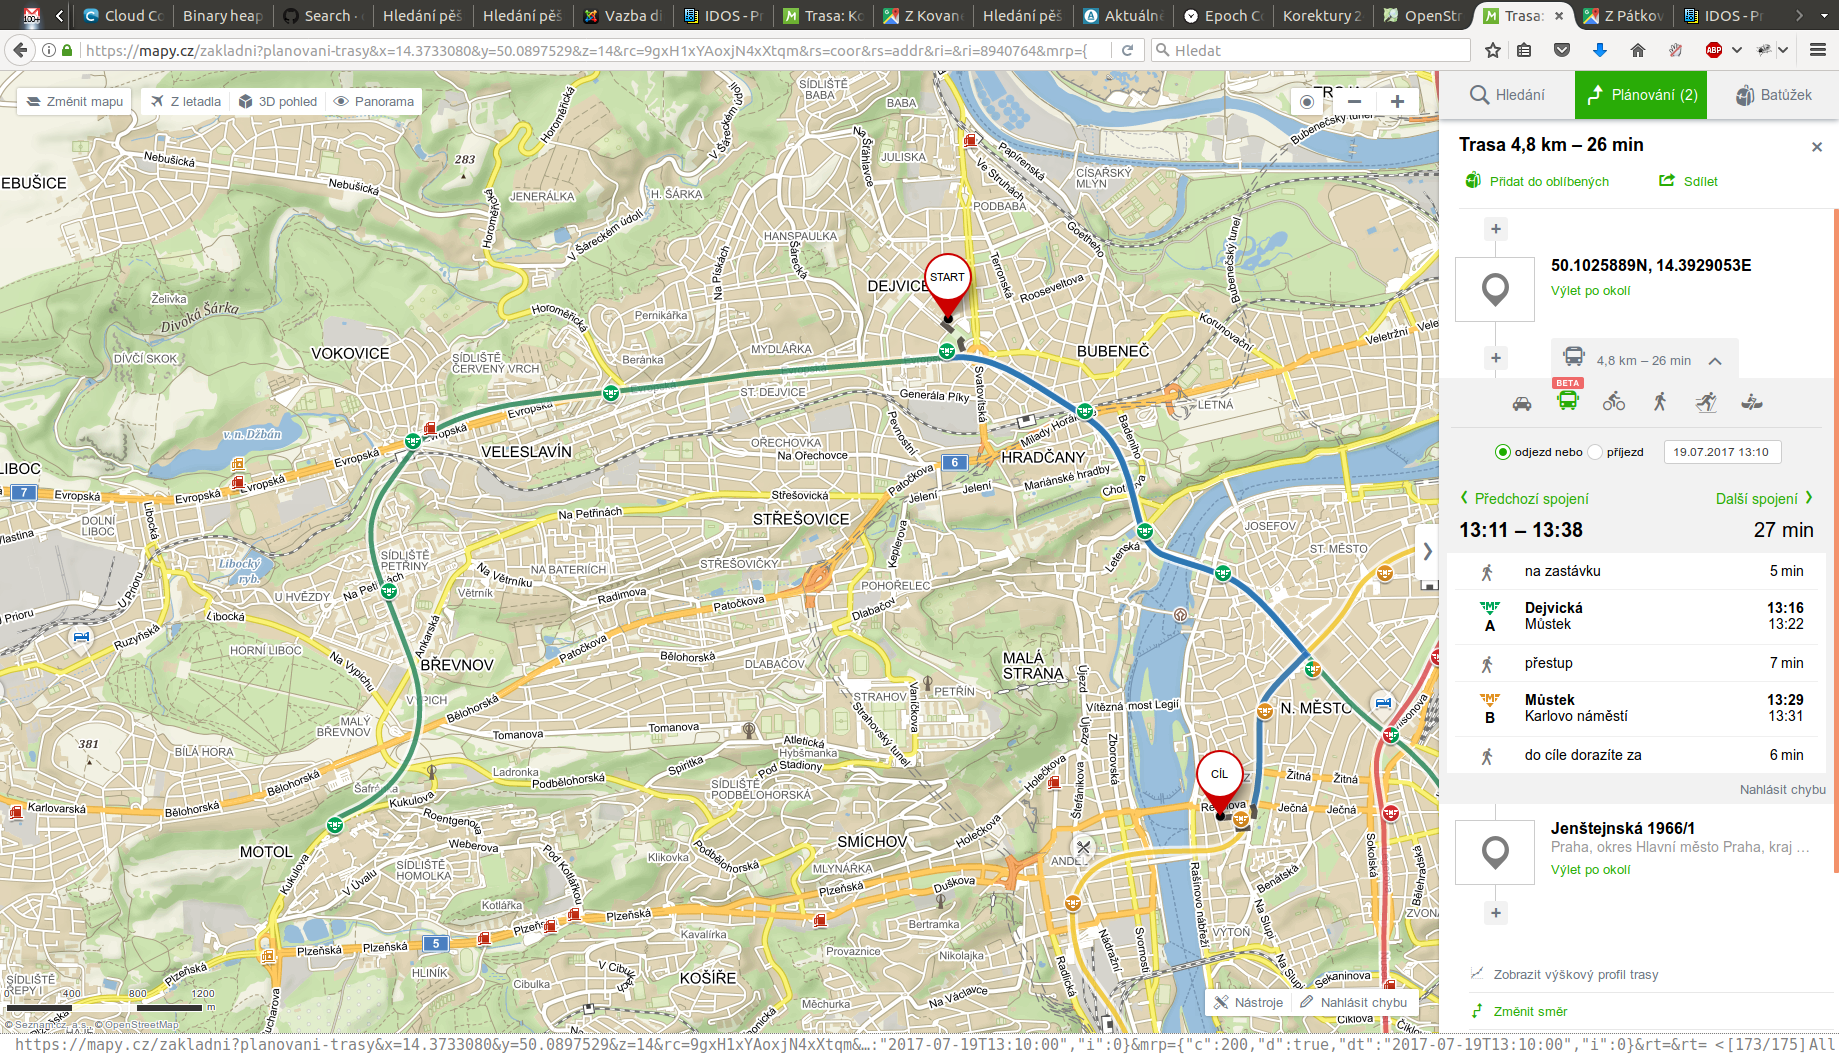
\includegraphics[width=\textwidth]{../img/fel-hlavkova-seznam.png}
  \caption{Spojení FEL ČVUT -- Hlávkova kolej podle Mapy.cz}
  \label{fig:fel-hlavkova-seznam}
\end{figure}
\begin{figure}[h]
  \centering
    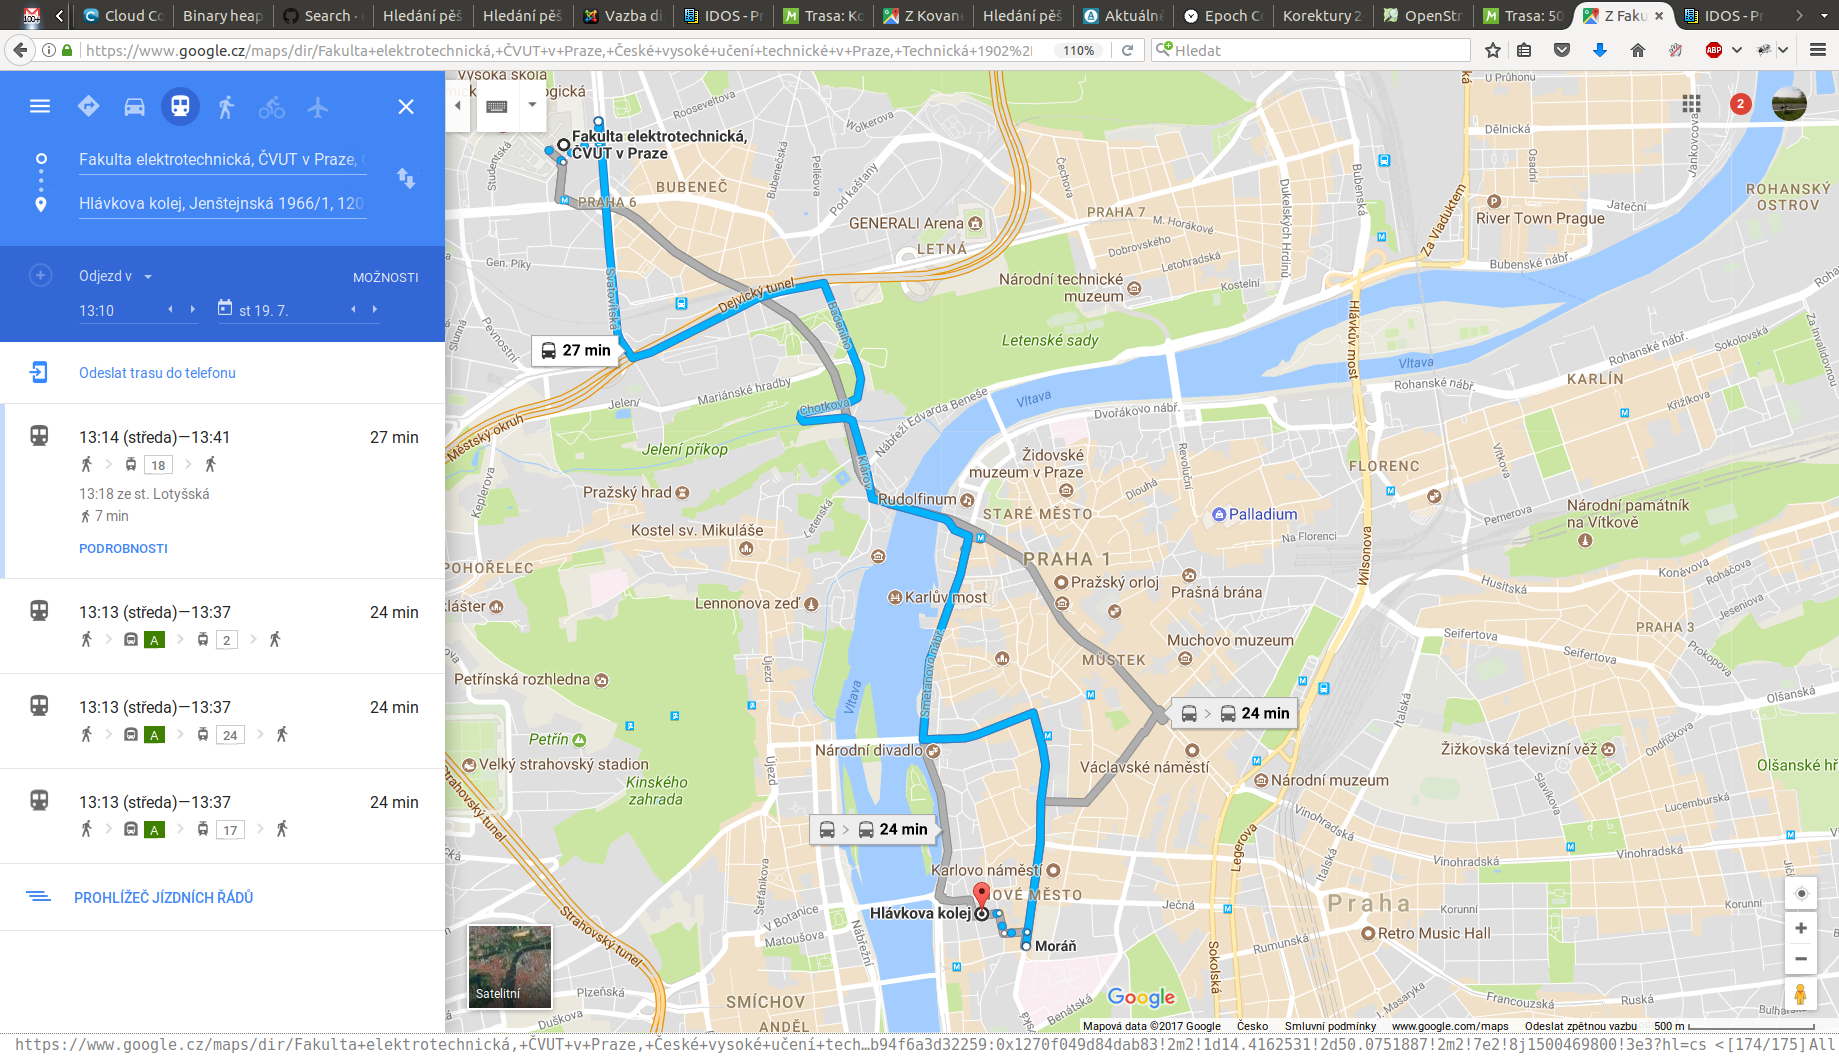
\includegraphics[width=\textwidth]{../img/fel-hlavkova-google.png}
  \caption{Spojení FEL ČVUT -- Hlávkova kolej podle Google Maps}
  \label{fig:fel-hlavkova-google}
\end{figure}

\clearpage
\section{Porovnání různých nastavení}
Pro porovnání různých nastavení našeho vyhledávače jsme zvolili trasu Kolej
17.listopadu -- Albertov, protože tato trasa poskytuje několik různých
alternativ spojení, tudíž jsme předpokládali, že se tyto alternativy projeví
v~nalezených trasách. Všechna spojení byla hledána od stejného času, pracovní den
v~brzkém odpoledni, tudíž by měl být eliminován vliv návazností, které fungují
jen v~určité minuty, protože podmínky jsou pro všechna hledání stejné.

Porovnávali jsme tato nastavení:
\begin{itemize}
	\item {\em Standardní}\\Základní nastavení vyhledávače, měl by se chovat
	obdobně jako jiné webové vyhledávače
	\item {\em Bez autobusu 201}\\ Linka 201 je ve směru z~kolejí na Nádraží
	Holešovice tak nespolehlivá, že je lepší s~ní vůbec nepočítat. Toto
	nastavení ji pomocí penalty {\tt inf} vyřazuje z~hledání.
	\item {\em Penalizace autobusů}\\ Test na penalizaci typu dopravního
	prostředku, měl by se snažit vyhýbat spojení autobusem a hledat jiné
	alternativy.
	\item {\em Jen jeden spoj}\\ Test na hledání, kterým spojem jet, pokud
	nechceme nikde přestupovat.
	\item {\em Pouze pěšky}\\ Ačkoli je vyhledávač stavěn na kombinované hledání
	pěších přesunů a cest MHD, stále by měl umět najít i pouze pěší cestu.
	\item {\em Na kole}\\ Tento test předpokládá jízdu na skládacím kole nebo
	koloběžce, tedy něčem, co lze vzít s~sebou do MHD. Testuje nestandardní
	vyhledávací parametry.
	\item {\em Penalizace pěších přesunů}\\ Opak předchozího testu, snažíme se
	minimalizovat pěší přesuny a co nejvíce se pohybovat pomocí MHD.
\end{itemize}
\subsection{Standardní}
Vyhledávání dle základního nastavení, které se nachází v~repozitáři v souboru {\tt
config/speeds.yaml}. U~ostatních testů bude uveden pouze rozdíl oproti tomuto
nastavení.

Trasa nalezená vyhledávačem se standardním nastavením je již popsána výše na
obr. \ref{fig:kolej-albertov-standard}, nebudeme ji zde znovu rozebírat.
\subsection{Bez autobusu 201}
Oproti standardnímu nastavení je pouze penalizace linky 201 nastavena na {\tt
inf}, tato linka by tedy k~hledání vůbec neměla být použita.

\begin{figure}[h]
  \centering
    \includegraphics[height=0.98\textheight]{../img/kolej-albertov-bez201.pdf}
  \caption{Spojení nevyužívající autobus 201}
  \label{fig:kolej-albertov-bez201}
\end{figure}

Vyhledávač nalezl mnoho různých tras. Trasy s~číslem menším než 12 mají příjezd
do 14:05, zbylé pak do 14:15. Zajímavé jsou pro nás trasy 0 a 1, protože zbylé
rychlé trasy jsou jen variacemi těchto tras. Trasa 0 odpovídá trase nalezené
standardním vylhedáváním, ale na Nádraží Holešovice využívá pěší přesun. Trasa 1
poněkud netradičně využívá přestup na linku 14 na Florenci s~pěším přesunem na
Těšnov. Ve výsledcích jsou i linky, které využívají možnosti dojet na Vyšehrad a
pak sejít do nuselského údolí z~druhé strany.

\subsection{Penalizace autobusů}
Oproti standardnímu nastavení mají autobusy fixní penaltu nastavenou na 100 a za
každou sekundu v~autobuse dostanou penaltu dalších 10. 

\begin{figure}[h]
  \centering
    \includegraphics[height=0.98\textheight]{../img/kolej-albertov-bus-penalta.pdf}
  \caption{Spojení penalizující autobusy}
  \label{fig:kolej-albertov-bus-penalta}
\end{figure}

Vyhledávač opět nalezl několik alternativ, které jsou velmi podobné předchozímu
vyhledávání. Je zde navíc varianta využívající dlouhý přesun tramvají č. 17
z~Trojské na Palackého náměstí a tam přestoupit do tramvaje na Albertov, která je
i podle zkušeností rychlá a spolehlivá. Všechny cesty na Trojskou a Nádraží
Holešovice v~této variantě jsou pěšky z~důvodu penalizace autobusů. 

\subsection{Jen jeden spoj}
Oproti standardnímu nastavení je počet nástupů do vozidla omezen na 1.

\begin{figure}[h]
  \centering
    \includegraphics[height=0.98\textheight]{../img/kolej-albertov-jeden-spoj.pdf}
  \caption{Spojení využívající nejvýše 1 spoj MHD}
  \label{fig:kolej-albertov-jeden-spoj}
\end{figure}

Nalezené spojení je vedeno tramvají č. 17 z~Trojské na Výtoň, odkud je to
na Albertov nejblíže. Cesta na Nádraží Holešovice a pak pěšky z~I. P. Pavlova
byla pravděpodobně delší a proto bylo toto spojení majorizováno.

\subsection{Pouze pěšky}
Oproti standardnímu nastavení je počet nástupů do vozidla omezen na 0.
\begin{figure}[h]
  \centering
    \includegraphics[height=0.98\textheight]{../img/kolej-albertov-pesky.pdf}
  \caption{Spojení pouze pěšky}
  \label{fig:kolej-albertov-pesky}
\end{figure}

Vyhledávač úspěšně nalezl pěší spojení až na Albertov, které by bylo
zvládnutelné, i když by to oproti cestě MHD trvalo výrazně déle. Při tomto
hledání byl vyhledávač výrazně pomalejší než pro kombinovaná spojení, což bylo
pravděpodobně způsobeno jednak mnohem větším stavovým prostorem, který bylo
potřeba projít, protože cesta trvá výrazně déle, jednak nutností zahazovat
všechna nalezená spojení pomocí MHD. Tomuto případu bychom mohli výrazně pomoci
tím, že bychom přepnuli na pouze pěší vyhledávač, ale neočekáváme, že by byly
často hledány pouze pěší trasy, proto jsme se rozhodli kód dále nerozšiřovat.

Na začátku trasy nalezl vylhedávač dvě alternativní trasy, jednu vedoucí horními
Holešovicemi přes kopec a druhou vedoucí po okraji dolních Holešovic podél
Argentinské. Ačkoli obě trasy jsou jistě zvládnutelné pěšky, ani jednu bychom si
pravděpodobně pro průchod holešovicemi nevybrali. První varianta obsahuje
zbytečné stoupání do kopce a pak klesání zpět k~Vltavě, což by se dalo omezit
nastavením délkového prodloužení za kopce, problém druhé cesty, dlouhou
procházku podél čtyřproudé silnice bychom v~současném stavu odstranit
nedokázali. Trasa je vedena po chodnících, tudíž penalty za silnice se
neuplatňují, bylo by potřeba při přípravě dat zjišťovat pro každou cestu objekty
v~jejím bezprostředním okolí a podle toho jí přidávat atributy, na které by se
pak dal brát ohled. Toto by však bylo výpočetně náročné a je to mimo rozsah této
práce.

\subsection{Na kole}
Oproti standardnímu nastavení byly přenastaveny rychlosti pohybu na rychlosti
mezi 10 a 25 km/h (mimo schodů, kde byly nastaveny 2km/h). Rovněž byly
penalizovány cesty do kopce (10\,m délky za metr převýšení) a zvýhodňovány cesty
z~kopce (-10\,m délky za metr převýšení). Navíc byla nastavena penalta za nástup
do vozidla na 100.

\begin{figure}[h]
  \centering
    \includegraphics[height=0.98\textheight]{../img/kolej-albertov-kolo.pdf}
  \caption{Spojení na kole}
  \label{fig:kolej-albertov-kolo}
\end{figure}

Toto vyhledávání byl spíše experiment, jak se bude vyhledávač chovat, pokud
nastavíme rychlosti výrazně výš než je obvyklá rychlost chůze. Pro vyhledávání
cyklistických tras není ve standardní konfiguraci vyhledávač vhodný, protože
klasifikuje objekty s~ohledem na pěší chůzi. Pro hledání cyklistických tras by
bylo potřeba výrazně pozměnit klasifikaci objektů, zařadit například typ povrchu
silnic a pravděpodobně zahodit zkratky, protože na kole nebývají potřeba a
nemusí být tak snadno realizovatelné. V~neposlední řadě existuje mnoho
kvalitních cyklistických vyhledávačů, které dávají výrazně kvalitnější výsledky
s~podobnou či lepší mírou přizpůsobení, například
BRouter\footnote{\url{http://brouter.de}}.

Vyhledané trasy odpovídají očekáváním s~ohledem na klasifikaci objektů. Všechny
vyhledané trasy využívají metro z~Nádraží Holešovice, liší se výstupní stanicí,
kterou je buď Hlavní Nádraží, I. P. Pavlova nebo Vyšehrad. Všechny trasy by
pravděpodobně byly průjezdné, ale překvapivě se na všech trasách nachází schody,
na kterých byla nastavena rychlost na 2 km/h a tudíž se je vyplatí objet. Pro
pohodlnější cesty by bylo vhodné přidat za schody i penaltu. Ověřenou
nejrychlejší cestu z~Vyšehradu, a to klesání ulicí Čiklovou a pak prokličkování
ulicí Na Slupi vyhledávač nenašel, protože v~současné klasifikaci by bylo těžké
popsat vhodně rychlostní profily jednotlivých druhů komunikací a hlavně povrchů.
Dlažba na trasách vedených mimo Vyšehrad činí tyto trasy výrazně pomalejší a
velmi nepohodlné.

\subsection{Penalizace pěších přesunů}
Pěší přesun po jakémkoli typu cesty je penalizován 100 za každou sekundu
strávenou pěším přesunem.

\begin{figure}[h]
  \centering
    \includegraphics[height=0.98\textheight]{../img/kolej-albertov-pesi-penalty.pdf}
  \caption{Spojení penalizující pohyb pěšky}
  \label{fig:kolej-albertov-pesi-penalty}
\end{figure}

Při tomto hledání je dobře vidět princip majorizovaných tras. Je nalezena
nejrychlejší trasa, ale protože obsahuje dlouhé pěší přesuny, má vysokou
penaltu. Proto se projeví i cesty časově výrazně delší, které ale využívají více
přesunů pomocí MHD a tedy mají nížší penaltu a nejsou majorizovány. Celkem
vyhledávač nalezl čtyři základní cesty a pak další, které se však od těchto
základních liší jen drobnými detaily. Nejkratší nalezená cesta má penaltu
přibližně 86\,000, trasa 30 má penaltu nejnižší a to přibližně 12\,300. 

\section{Profilování}
Jak jsme ověřili v~předchozí části, náš vyhledávač dává výsledky srovnatelné
s~ostatními dostupnými vyhledávači spojení a má široké možnosti konfigurace.
Rychlost vyhledávání spojení je však nízká, středně dlouhá spojení přes střed
města hledá v~jednotkách sekund, při specifických konfiguracích (například pouze
pěší vyhledávání) jsou ale časy výrazně delší, dosahují i desítek sekund.
Ačkoliv rychlost nebyla našim hlavním cílem, pro praktické nasazení je nezbytné,
aby vyhledávač pracoval co nejrychleji. 

Abychom zjistili, kde se při hledání tráví největší čas, profilovali jsme
vyhledávač pomocí aplikace {\tt perf}. Abychom eliminovali vliv načítání mapy a
jízdního řádu, což se při běžném vylhedávání děje jen jednou při spuštění webové
aplikace, vytvořili jsme testovací scénář pro konzolovou aplikaci. Ta si nejprve
načetla mapová data a data jízdních řádů a potom postupně hledala různá spojení
mezi předem zvolenými body. Nasbíraná data jsme pak analyzovali a na jejich
základě provedli některé optimalizace, například vyhazování majorizovaných
položek z~haldy a seznamu vrcholů.

Z~naměřených dat vyplývá, že místo, kde by se mělo optimalizovat nejdříve, je
cyklus porovnávající, zda právě přidávaná položka do haldy není majorizována či
naopak majorizuje nějakou jinou položku, která už v~haldě je. Ve standardním
nastavení se v~tomto cylku stráví okolo 25\,\% času, při hledání pouze pěších
tras je to až 50\,\%. Dalším místem v~pořadí je načítání pěší hrany při
zpracovávání vrcholu a zjišťování, který její konec máme uvažovat. Zde si
myslíme, že dochází ke zpomalení převážně z~důvodu přístupu na náhodné místo
v~paměti, protože hran je mnoho a nejsou nijak setříděné. Překvapivě velký čas je
zabrán počítáním penalty bodu. I~když se jedná o~funkci obsahující pouze 2
podmínky, tráví se zde 6\,\% celkového času, což nám přišlo zvláštní, ale nemáme
pro to jasný důvod. Posledním významným časem je hledání minima v~haldě, což je
ale logaritmická operace a proto nás 7\,\% stráveného času příliš nepřekvapí.



\chapter*{Závěr}
\addcontentsline{toc}{chapter}{Závěr}

zrychleni - potencialova heuristika, viz MJ - skripta z GA

skriptovani vypoctu penalt

Další možné rozšíření systému penalt by mohlo být například posuzování intervalů
linek, kdy bychom mohli preferovat častěji jedoucí linky. 

posun odchodu podle prvniho MHD

okolí cest


%%% Seznam použité literatury
%%% Seznam použité literatury je zpracován podle platných standardů. Povinnou citační
%%% normou pro bakalářskou práci je ISO 690. Jména časopisů lze uvádět zkráceně, ale jen
%%% v kodifikované podobě. Všechny použité zdroje a prameny musí být řádně citovány.

\def\bibname{Seznam použité literatury}
\begin{thebibliography}{99}
\addcontentsline{toc}{chapter}{\bibname}

\bibitem{lamport94}
  {\sc Lamport,} Leslie.
  \emph{\LaTeX: A~Document Preparation System}.
  2. vydání.
  Massachusetts: Addison Wesley, 1994.
  ISBN 0-201-52983-1.

\bibitem{osmweb}
	\emph{OpenStreetMap} [online]. 
	2014, 4.5.2014 [cit. 2014-05-04]. 
	Dostupné z: \url{http://www.openstreetmap.org}

\bibitem{osmxml}
	\emph{OSM XML} [online]. 
	2014, 16 September 2013 [cit. 2014-05-06]. 
	Dostupné z: \url{http://wiki.openstreetmap.org/wiki/OSM_XML}

\bibitem{osmfeatures}
	\emph{Cs: Map Features} [online]. 
	2014-04-01 [cit. 2014-05-17]. 
	Dostupné z: \url{http://wiki.openstreetmap.org/wiki/Cs:Map_Features}

\bibitem{wgsnorma}
	{\sc NIMA.}
	\emph{World geodetic system 1984} [online]. 
	3. vydání, 1. dodatek.
	3 January 2000 [cit. 2014-05-04]. 
	Dostupné z: \url{http://www2.jpl.nasa.gov/srtm/}.

\bibitem{utmnorma}
	{\sc Snyder,} John P.
	\emph{Map Projections: A~Working Manual} [online]. 
	1987, [cit. 2014-05-08]. 
	Dostupné z: \url{http://pubs.er.usgs.gov/publication/pp1395}.

\bibitem{srtmweb}
	{\sc NASA.}
	\emph{The Shuttle Radar Topography Mission} [online]. 
	2014, June 17, 2009 [cit. 2014-05-04]. 
	Dostupné z: \url{http://www2.jpl.nasa.gov/srtm/}.

\bibitem{pbfweb}
	{\sc Google.}
	\emph{Protocol Buffers} [online]. 
	2014, April 2, 2012 [cit. 2014-05-05]. 
	Dostupné z: \url{https://developers.google.com/protocol-buffers/}.

\bibitem{pbfenc}
	{\sc Google.}
	\emph{Encoding - Protocol Buffers} [online]. 
	2014, April 2, 2012 [cit. 2014-05-07]. 
	Dostupné z: \url{https://developers.google.com/protocol-buffers/docs/encoding}.

\bibitem{pbfspec}
	{\sc Google.}
	\emph{Language Guide - Protocol Buffers} [online]. 
	2014, April 22, 2014 [cit. 2014-05-07]. 
	Dostupné z:	\url{https://developers.google.com/protocol-buffers/docs/proto}.

\bibitem{lineint}
	{\sc Weisstein} Eric W.
	\emph{Line-Line Intersection.} [online]. 
	2014, May 12, 2014 [cit. 2014-05-12]. 
	Dostupné z:	\url{http://mathworld.wolfram.com/Line-LineIntersection.html}.

\bibitem{zametani}
	{\sc Mareš} Martin
	\emph{Geometrické algortimy} [online]. 
	2014, 17.11.2013 [cit. 2014-05-13]. 
	Dostupné z:	\url{http://mj.ucw.cz/vyuka/ads/43-geom.pdf}.
	

\end{thebibliography}


%%% Obrázky v diplomové práci
%%% (pokud jich je malé množství, obvykle není třeba seznam uvádět)
\listoffigures

%%% Tabulky v diplomové práci (opět nemusí být nutné uvádět)
%%% U matematických prací může být lepší přemístit seznam tabulek na začátek práce.
\listoftables

%%% Použité zkratky v diplomové práci (opět nemusí být nutné uvádět)
%%% U matematických prací může být lepší přemístit seznam zkratek na začátek práce.
\chapwithtoc{Seznam použitých zkratek}

%%% Přílohy k diplomové práci, existují-li. Každá příloha musí být alespoň jednou
%%% odkazována z vlastního textu práce. Přílohy se číslují.
%%%
%%% Do tištěné verze se spíše hodí přílohy, které lze číst a prohlížet (dodatečné
%%% tabulky a grafy, různé textové doplňky, ukázky výstupů z počítačových programů,
%%% apod.). Do elektronické verze se hodí přílohy, které budou spíše používány
%%% v elektronické podobě než čteny (zdrojové kódy programů, datové soubory,
%%% interaktivní grafy apod.). Elektronické přílohy se nahrávají do SISu a lze
%%% je také do práce vložit na CD/DVD. Povolené formáty souborů specifikuje
%%% opatření rektora č. 13/2017.
\appendix
\chapter{Přílohy}

\section{První příloha}

\openright
\end{document}
